\chapter{Co-Lab: Community-based Load Balancing Approach}\label{Chap5}
\echapter{Co-Lab: Community-based Load Balancing Approach}

\section{Introduction}\label{Chap5_01}
\esection{Introduction}
In socially-aware networking environments, users generate large amounts of data by exploiting capability-rich mobile devices, and prefer to share with people they have social relationships or similar interests with. However, data dissemination in this setting posses a difficult problem~\cite{YZhu2013}. As the topology is very unstable, and users appear in and disappear from the network dynamically, event producers and consumers might never connect at the same time to a given network. Therefore, data objects should be moved and replicated in the community in order for the effective delivery to interested users.  Several solutions have been proposed that consider the interest similarity of brokers and attempt to cluster brokers in such a way that the notification delay and other involved costs are minimized. For instance,  Fig. 5.1 presents an example of a dynamic solution for publish/subscribe systems. The publisher advertises an event and subsequent subscriptions are connected with the producer. Then, a consumer system relocates from broker A to broker B. After that, the topology needs to be updated in order to ensure that the event flows to broker B. Once the topology has been updated, the old subscription can be removed if there are no other subscribers at broker A.

Event-based publish/subscribe systems have been widely used in large-scale distributed applications because it allows processes to communicate asynchronously in a loosely and decoupled manner. This property gives networking systems higher modularity and re-usability as well as easier maintainability.
\begin{figure}[h]
\begin{center}
  \begin{tabular}{c}
  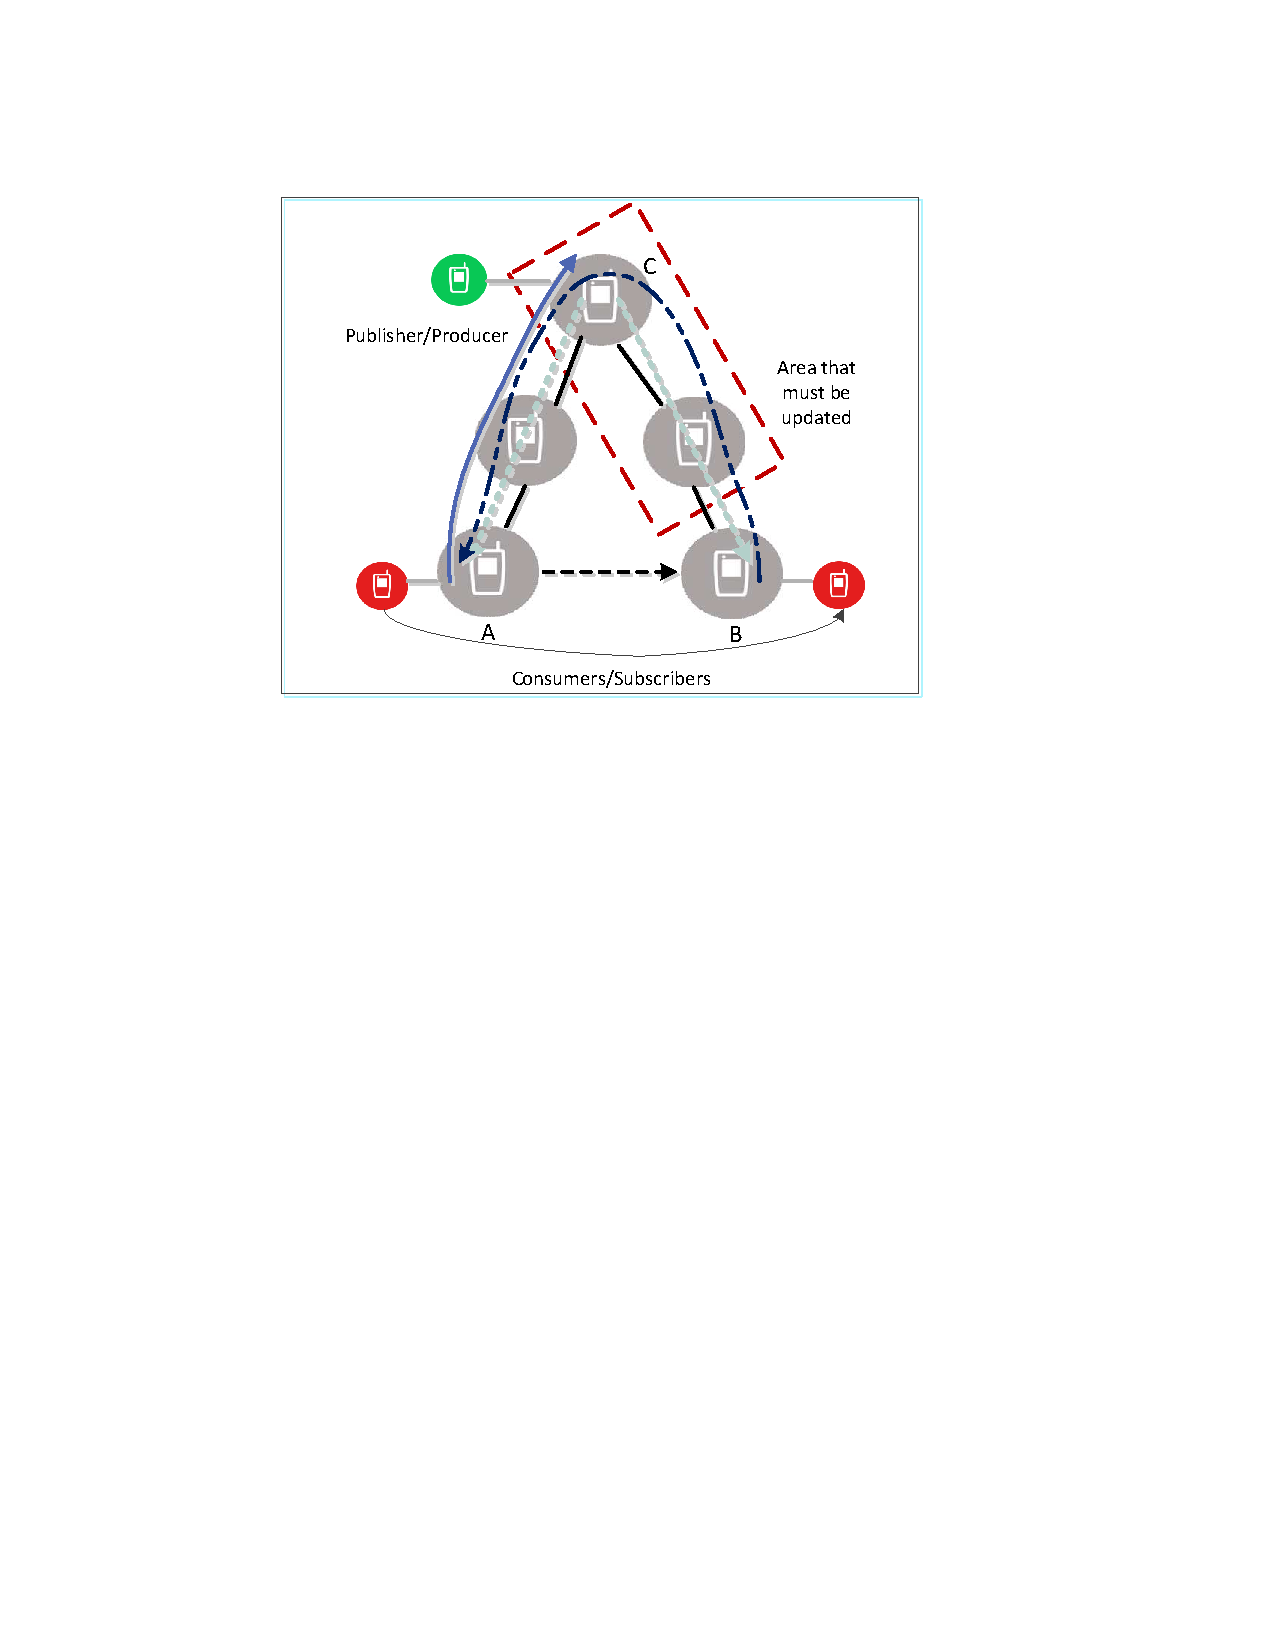
\includegraphics[width=0.5\textwidth]{Chap5-Fig1.pdf}
  \end{tabular}
  \caption{An example of publish/subscribe systems dynamic solution.}
\end{center}
\end{figure}
In publish/subscribe systems, loose-coupling is achieved by allowing producers to publish information in the network without knowing the identity, location, and number of subscribers. Likewise, consumers subscribe to specific information without knowing the identity, location, and number of publishers. Thus, the matching rate of both the publication and subscription determines the load of a broker~\cite{AKYCheung2010}. In turn, these factors depend on the number and nature of subscriptions that the broker serves. Therefore, load balancing is possible by offloading subscriptions from higher loaded to lesser loaded brokers. Although, load balancing has been a widely explored research topic for the past two decades, the existing offloading mechanisms do not address most of the challenges such as reducing the overall load distribution and fault-tolerance.  To the best of our knowledge, we are among the first to address load balancing and reliability by exploiting fault-tolerance techniques in event-based publish/subscribe systems.

The computing power of any distributed system can be realized by allowing its constituent computational elements, brokers or nodes, to work cooperatively so that large loads are allocated among them in a fair and effective manner. Any strategy for load distribution among these elements is called load balancing. An effective load balancing policy ensures optimal use of the system resources whereby no broker remains in an under-loaded state while any other broker is being highly utilized or overloaded. Not limited to socially-aware networks, in many today's distributed environments, the computers are linked by a delay and bandwidth is limited by communication medium that inherently inflicts tangible delays or inter-resource communications and load exchange~\cite{SDhakal2007}. To be able to fully benefit from such networking systems, resource management, data availability and reliability are key services, where issues of load balancing, partitioning and fault tolerance present a common challenge.

Recently, there has been a great effort to design and develop load balancing algorithms and fault tolerant mechanisms that are capable of improving the performance, reliability and flexibility of networking systems. Unfortunately, many practical instances of the load balancing problems have been found to be NP-complete~\cite{XZhu2011}. Hence, our work is motivated by the need for efficient algorithms which considers community formation, event dissemination, broker clustering based on interest similarity, replication, load distribution and fault-tolerance. Our main objective is to arrive at load distributions that will achieve minimum load difference between the overloaded and under-loaded brokers even during resource or link failure thereby resulting in reduced overall load distribution and a greater degree of fault-tolerance. In this chapter, we focused on designing optimal community-based load balancing and event forwarding algorithm (Co-Lab) with inspiration taken from community-based and cluster-based load balancing approaches.

The rest of this chapter is organized as follows. Related work is discussed in~\ref{Chap5_02}. \ref{Chap5_03} discusses our preliminary design. \ref{Chap5_04} discusses Co-Lab, our community-based load balancing approach. \ref{Chap5_05} presents the performance evaluation results which are analyzed and discussed, followed by a section (\ref{Chap5_06}) dedicated to conclusion and future work.

\section{Related Work}\label{Chap5_02}
\esection{Related Work}
Most of data dissemination and forwarding systems that use tree-based, DHT-based or cluster-based approaches do not provide any load balancing mechanism. Cheung and Jacobsen~\cite{AKYCheung2010} proposed a new load balancing algorithm that distributes load by offloading strategically chosen subscriptions from heavily loaded brokers to less loaded brokers. On the other hand, Zhang {\it et al.}~\cite{HZhang2008} presented the design of Shuffle, an active workload management middleware to support a scalable broker network. Shuffle offers an integral solution to manage all types of the workload in a pub/sub broker network within a single overlay topology. The need of energy efficiency is a problem concerning the constraints imposed by battery capacity and heat dissipation which are opposed by the desire of miniaturization and portability. Motivated by this observation, an energy saving and load balancing routing technique was proposed in the work of Rango and Tropea~\cite{FDeRango2009}, using a novel pheromone updating policy based on multiple performance metrics. There are a couple of existing research works that represents a first step towards the realization of a complete solution for load balancing in a cooperative, distributed environment such as kim {\it et al.}~\cite{SManfredi2013} and Manfredi {\it et al.}~\cite{HKim2012}.

Resource failures may frequently occur in socially-aware networks and have adverse effect on applications. Consequently, there is an increasing need for employing techniques to achieve fault tolerance. Therefore, fault tolerance can be provided by partitioning the network in to communities and allocating replicas of the event to those communities~\cite{Pujol2010}\cite{SGitzenis2013}\cite{MYuan2012}. Partitioning can improve availability, by ensuring that when one partition fails the remaining partitions are able to answer some of the subscriptions, and increase manageability. However, according to Curino {\it et al.}~\cite{CCurino2010}, it will not be able to predict future queries in the networks, when both data and network are changing over time. There are valuable works regarding data replication, while also guaranteeing a fair load balancing at the nodes have been tried to be addressed in our previous chapter (ComPAS) and some other existing works such as Lang {\it et al.}~\cite{WLang2010} and La {\it et al.}~\cite{CALa2012}. However, the load balancing methods they exploited are not mentioned explicitly in their work.


\section{Preliminaries}\label{Chap5_03}
\esection{Preliminaries}

\subsection{Community Partitioning}\label{Chap5_03_01}
\esubsection{Community Partitioning}

Social community can be created based on similar characteristics of individuals, including physical and social characteristics. In some cases, communities can be formed in advance; while in other cases, communities are dynamic and can only be created progressively. The specific approach for the creation of social communities depends on initiators' social goals~\cite{DZhang2011}. In this section we focus on structuring the system into communities.

We assume the network system consists of a set of brokers, $B=\{B_1,..., B_n\}$. Brokers communicate through reliable TCP links and have unique identification numbers. There are two main questions that should be answered in creating and structuring social communities. 1) How many social communities should be in the system? 2) How many brokers should be in each community? The answer for these questions directly affects the performance of the proposed load balancing approach experienced by a single broker and overall network traffic for dissemination of subscriptions and publications. Assuming subscriptions and publications of events are distributed uniformly among brokers, we want to structure communities in such a way that load distribution is uniform among brokers. We believe that this can be achieved if the sizes of communities are the same. It is straightforward to show that if the sizes of communities differ significantly, the distribution of loads among brokers will not be uniform. Fig. 5.2 displays a sample of socially-aware network structured into three communities.
\begin{figure}[t]
\begin{center}
  \begin{tabular}{c}
  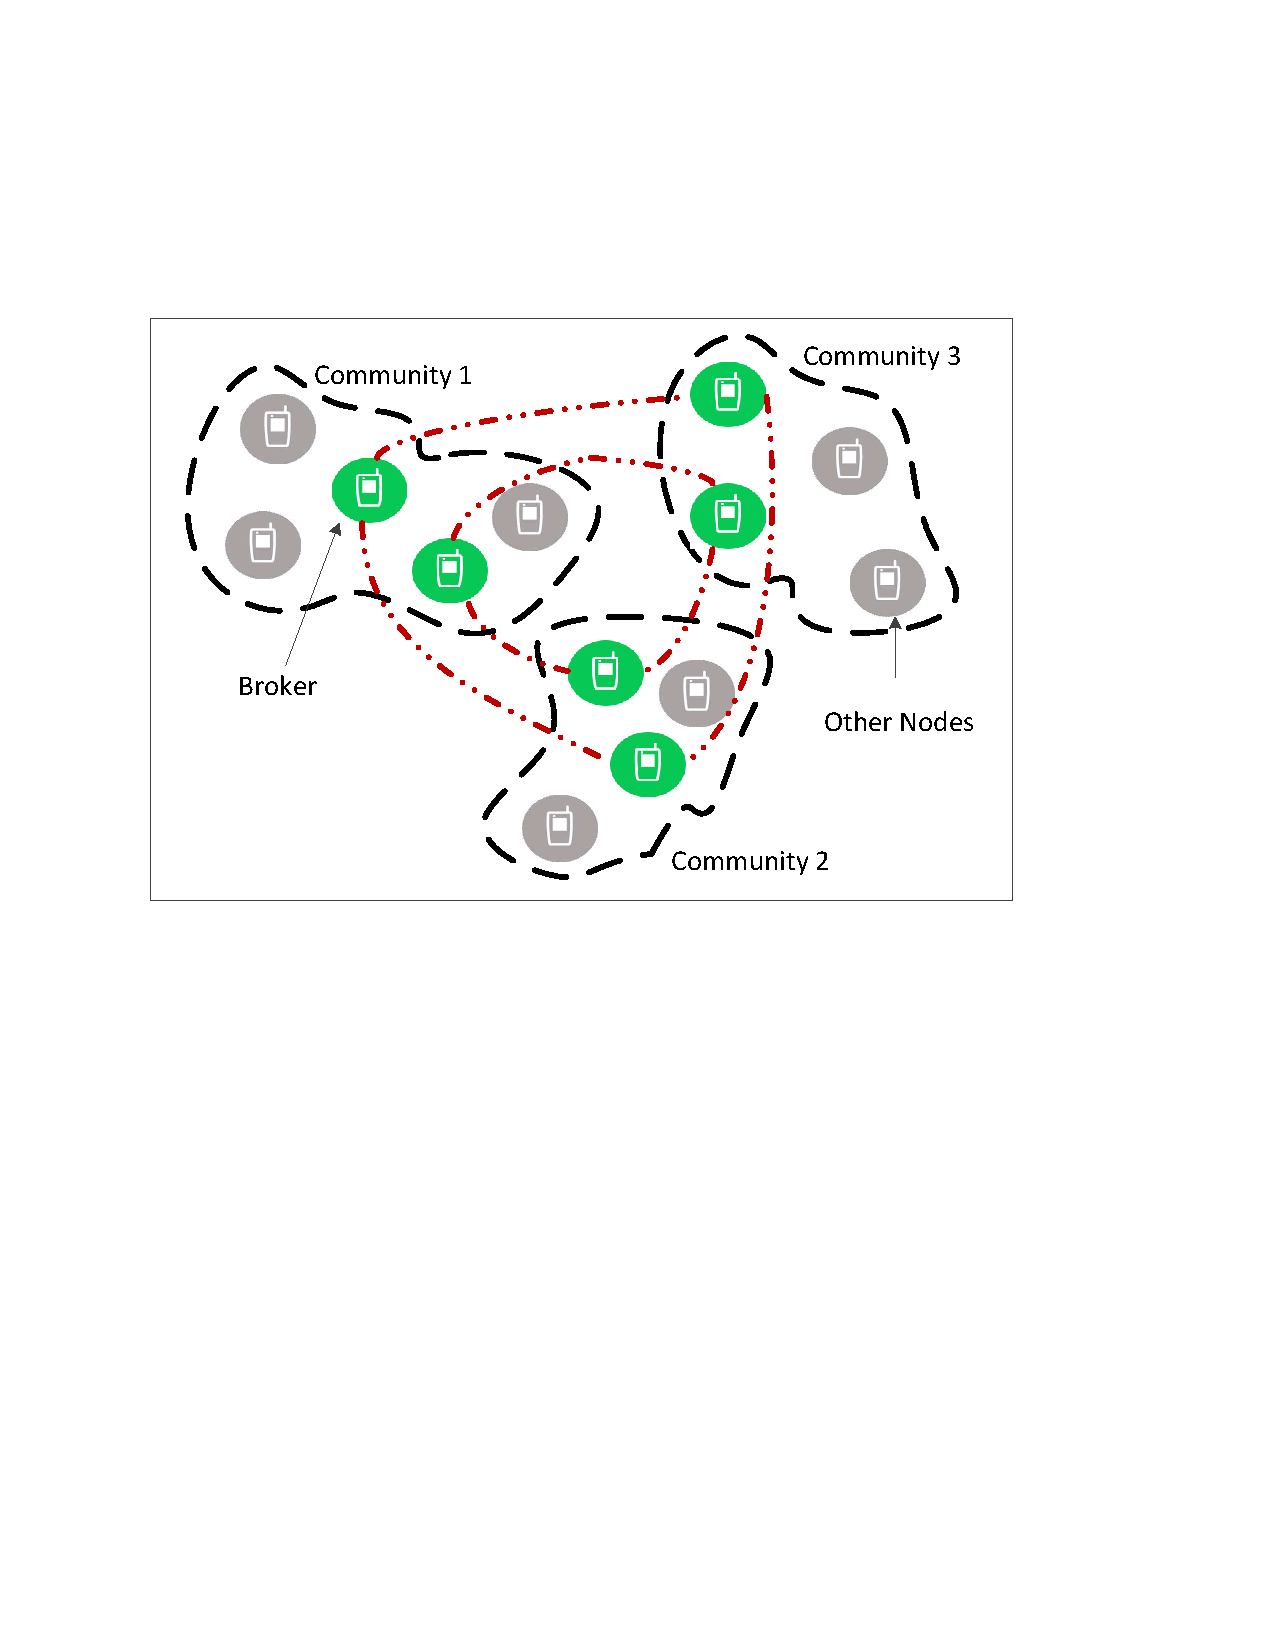
\includegraphics[width=0.55\textwidth]{Chap5-Fig2.pdf}
  \end{tabular}
  \caption{Sample socially-aware network system with 6 brokers structured into 3 communities.}
\end{center}
\end{figure}

Therefore, at the beginning, the system tries to generate almost equal social communities. Assuming that the community sizes are equal, we will find the number of communities in the network system to achieve better performance through reducing overall network traffic resulted from dissemination of subscriptions and publications. In order to attain the goal, we first compute the overall network traffic in the system as follows.

Assume, there are $N$ brokers in the network system and we intend to structure them into $K$ social communities with equal sizes. The probability for a broker to have subscription matching with the advertizement or publication is $\ell(0\leq\ell\leq1)$, where $\ell$ represents the matching ratio.
\begin{equation}
TNT=AT+CT.
\end{equation}

In Equation 5.1, TNT denotes the total network traffic, AT denotes publication forwarding traffic, and CT denotes the subscription forwarding traffic. Event publication is disseminated to $K-1$ communities, where $(K-1)$ is the event dissemination traffic which results in $(K-1)$ notifications or messages. At this phase, $K$ brokers have the published notifications. Considering matching ratio $\ell$, $\ell(N-K)$ brokers out of the remaining $(N-K)$ brokers have matching subscriptions and must receive the notification. This results in an extra $\ell(N-K)$ notifications. Therefore, the $AT$ resulted from one publication is $(K-1)+\ell(N-K)$.

If we have $A$ publications/advertisements with matching ratio $\ell$ in the network system, the overall publication traffic for matching ratio $\ell$ is $A[(K-1)+\ell(N-K)]$. Assuming publications are distributed uniformly for matching ratios, the overall publication traffic for all matching ratios is computed as follows.

\begin{eqnarray}
AT&=&\int_0^1[A(K-1)+A(N-K)\ell]d\ell \nonumber\\
AT&=&A(K-1)+\frac{A}{2}(N-K).
\end{eqnarray}

When we come to the overall subscription traffic, since subscriptions are only disseminated in a community, it can be computed as follows where $C$ is the total number of subscriptions in the network system.
\begin{eqnarray}
CT&=&C\left(\frac{N}{K}-1\right)\\
TNT&=&AT+CT \nonumber\\
TNT&=&A(K-1)+\frac{A}{2}(N-K)+C\left(\frac{N}{K}-1\right).
\end{eqnarray}

We assume that the overall network traffic ($TNT$) is a function of $K$, using the number of communities in the system, we can achieve the value of $K$ that results in the minimum $TNT$ as follows.

\begin{equation}
Number~of~communities=K=\sqrt{\frac{2C}{A}N}.
\end{equation}

This equation shows that the initial number of communities in the system has a direct relation with the number of subscriptions and an indirect relation with the number of publications. By considering the amount of publications is one-fifth of the amount of subscriptions our system uses 3($\sqrt{N}$) as the initial number of communities.

\subsection{Subscription Replicating}\label{Chap5_03_02}
\esubsection{Subscription Replicating}
Most of the existing load balancing approaches including the solution by Cheung and Jacobsen~\cite{AKYCheung2010} distributes load by offloading chosen subscriptions from heavily loaded brokers to less loaded brokers. Filter-based and multicast-based are the two existing main approaches of event-based publish/subscribe systems. In the filter-based approach, subscriptions are broadcasted into the network to establish routes that direct publications to subscribers. Each publication is matched at every broker along the overlay to get forwarded towards neighbors with matching subscriptions. In the multicast-based approach, subscribers with similar interests are grouped into the same multicast set. Each publication is matched once to determine the matching multicast group(s) to which the message should be multicasted, broadcasted, or unicasted. As a result, matching and transmission of a publication message happens at most once, thus incurring minimal delivery delay. However, compared to the filter-based approach, subscribers in a multicast group may receive unwanted publications because subscribers with even slightly different interests may still be assigned to the same group~\cite{FCao2004}. Based on this fact, we propose one possible solution to this problem by integrating filter-based functionality within each multicast group.

In an event-based publish/subscribe model, a multidimensional data space is defined on $d$ attributes. An event $E$ can be represented as a set of $<a_i, v_i>$ data tuples where $v_i$ is the value this event specifies for the attribute $a_i$. A subscription can be represented as a filter $\theta$ that is a conjunction of $k$ $(k \leq d)$ predicates, and each predicate specifies a constraint on a different attribute, such as "$a_i=X$", or "$X \leq a_i \leq Y$".

To make load balance between overloaded brokers $B^o$, we propose to replicate the filters in $B^o$ to a group of under-loaded brokers $B^u$ in the community. In order to make a replica of filter, we create a cluster of brokers such that all member brokers of the cluster can maintain the same filters. Hence, a cluster G of brokers contains $N$ brokers $B_i$ with $1 \leq i \leq N$. The union of two filters (i.e. $A$ and $B$) in the cluster is the collection of filters in both $A$ and $B$. ($A \cup B={x:x \in A~or~x \in B}$)

Sets of filters cannot have duplicate elements. For example: the union of ${1,2,3}$ and ${2,4}$ is ${1,2,3,4}$. Multiple occurrences of identical elements have no effect on the cardinality of a set or its content. The same is true for the union of filters in the cluster. Denote $\theta_i$ to be the filters maintained by $B_i$ before replication. After the implementation of replication for filters on the brokers in the cluster $G$, each broker in $G$ maintains the union of filter sets as $\theta_1 \cup \theta_2 ... \cup \theta_i$.

\begin{figure}[h]
\begin{center}
  \begin{tabular}{c}
  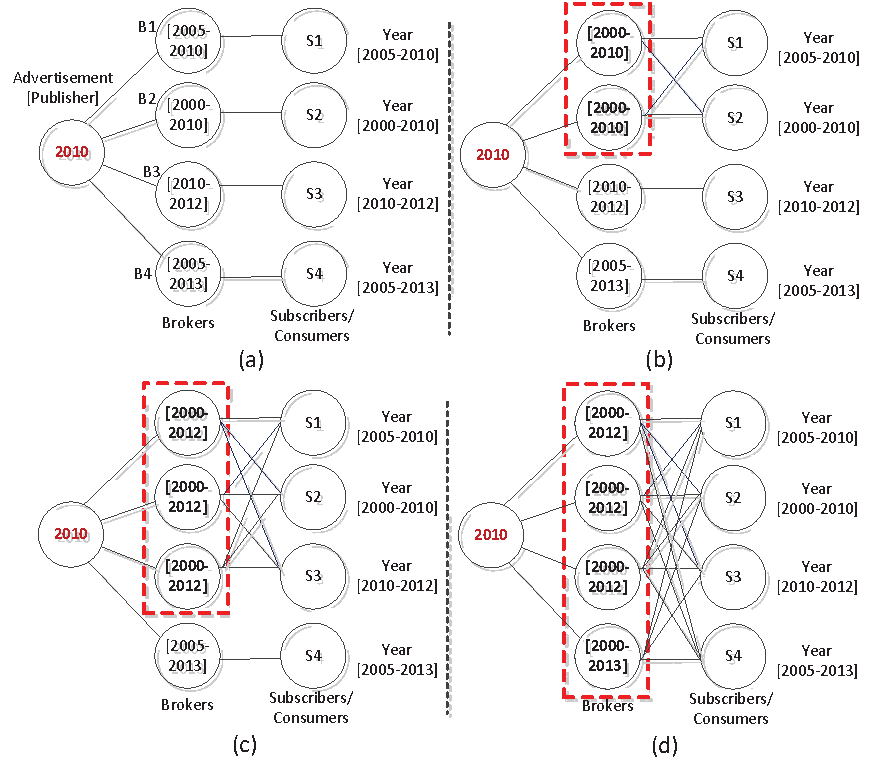
\includegraphics[width=0.8\textwidth]{Chap5-Fig3.pdf}
  \end{tabular}
  \caption{An example of social graph based interest replication with a) no replication; b) replicating interests on $B1$ and $B2$; c) replicating interests on $B1$, $B2$, and $B3$; d) replicating interests on $B1$, $B2$, $B3$, and $B4$.}
\end{center}
\end{figure}

Let's use Fig. 5.3 to illustrate the concept of our proposed filter replication. Consider a social graph using 1 publisher, 4 brokers and 4 subscribers. The brokers $B_1$, $B_2$, $B_3$ and $B_4$ are used to connect subscribers $S_1$, $S_2$, $S_3$ and $S_4$, respectively. In the figure, we assume that all filters/interests define predicates over an attribute $year$ (movie release year). For example, $S_1$ defines a filter to be a predicate with the $year$ inside the interval [2005-2010]. That means, $S_1$ is interested in movies released between 2005 and 2010 for that particular event. Fig. 5.3(a) shows the brokers $B_1$, $B_2$, $B_3$ and $B_4$ and the maintained filter before replication. Suppose that the publishers produce a large number of advertisements having the $year$ 2010. Denote $P$ to be the number of such publication. Then, following the forwarding protocol of the friendship based social graph, all four brokers $B_1$, $B_2$, $B_3$ and $B_4$ suffer from heavy work loads to receive such $P$ publications.

To overcome the above mentioned heavy load on brokers, in Fig. 5.3(b), we initially propose to replicate the filters of $B_1$ and $B_2$. In this way, $B_1$ and $B_2$ form a cluster and maintain exactly the same generalized filters (using Union operation) $\theta_1 \cup \theta_2 = {year: [2000-2010]}$. At the same moment, brokers $B_1$ and $B_2$ builds an extra link with $S_2$ and $S_1$ respectively. Now for each of the $P$ publications, the publisher randomly chooses one of the two brokers $B_1$ and $B_2$ with equal probability of 50\%, and then forwards the publication to the chosen broker. When receiving the forwarded publication, the downstream broker finally delivers the publication to the appropriate subscribers. The brokers $B_1$ and $B_2$ then equally receive on average $P$/2 publication/advertisements, yet $B_3$ and $B_4$ still receives $P$ publications.

Next, we need to balance the loads of three brokers, in Fig. 5.3(c), we replicate the filter of $B_1$, $B_2$ and $B_3$, such that all three brokers form a cluster and maintain the same filter $\theta_1 \cup \theta_2 \cup \theta_3 = {year: [2000-2012]}$. In addition to that, the brokers build extra links with the corresponding subscribers. Now, each of the brokers $B_1$, $B_2$ and $B_3$ equally receives on average $P$/3 publications. To further balance the loads of all the brokers in the social graph, in Fig. 5.3(d), we replicate the filter of $B_1$, $B_2$, $B_3$ and $B_4$ in the same procedure as explained above. As a result of the balancing operation on all the brokers, $B_1$, $B_2$, $B_3$ and $B_4$ equally receive publications with a probability of 25\%.

Apart from the balanced loads among brokers, the uniqueness of this replication is the reduction of overall publication loads by the proposed publication algorithms given in the next subsection. It is mentioned earlier that most of the existing solutions simply offload the loads from the overloaded brokers $B^o$ to under-loaded brokers $B^u$. These solutions do not lead to the reduction of overall number of publications and can cause sudden ways of offloading filters back-and-forth across the brokers in the community. For instance, consider that the load of an overloaded broker $B^o$ is offloaded to an under-loaded broker $B^u$. After that, when there exist publications matching the filters preserved by $B^u$, the broker $B^u$ becomes overloaded and the load of $B^u$ might be moved back to $B^o$. This condition can similarly occur on the broker $B^o$, leading to a sudden way of offloading filters back and forth onto $B^o$ and $B^u$. However, in the proposed filter replication approach, there is no need to move filters back and forth onto $B^o$ and $B^u$, which eliminates the sudden ways of offloading issue.

\subsection{Event Dissemination Algorithm}\label{Chap5_03_03}
\esubsection{Event Dissemination Algorithm}
The dissemination of event $E$ is done in two phases. The first phase is dissemination among different communities (Inter-Community) where a published event is broadcasted among all communities through the publisher broker's community link ($A_{InterCom}$). In the second phase, which is dissemination of event $E$ within the community (Intra-Community), the event is matched to subscriptions in each community and is delivered to the brokers with matching subscription. Upon receiving the incoming $E$, the selected broker matches $E$ with filters including replicated filters from other clustered brokers. If the matching filters are found, the selected broker then sends $E$ to the subscribers. As shown in Algorithm 3, we propose two optional approaches to select $B_i$ among the member brokers inside community $C$. In $random~approach$, each broker in community $C$ is evenly selected with the probability of $1/C$. This approach is improved through the $greedy~method$ by selecting the broker with the smallest load inside $C$. The formal representation of the event dissemination is depicted as follows.

\begin{algorithm}
  \Begin{
    $B_A \leftarrow$ The publisher broker\;
    $A_{InterCom} \leftarrow$ The publisher broker's community link\;
    {\bf Inter-Community Phase:}\\
     \For{$B_i \in A_{InterCom}$}{
            $B_A$ sends event $E$ to $B_i$;
     }
    {\bf Intra-Community Phase:}\\
     \For{$B_i \in A_{InteCom}$}{
            $B_i$ matches event $E$ with subscription in its community\;
            \If{event $E$ matches the subscriptions}{
               i- Select a broker $B_i$ randomly\;
               ii- Select a broker $B_i$ with the smallest load\;
               Send event $E$ to the selected broker
               }
            }
  }
\caption{Pseudocode for dissemination of event $E$}
\label{alg:chap5_alg01}
\end{algorithm}

When we come to the analysis of the loads of the brokers, there is no load change for those non-clustered brokers for the filter replication operation. Therefore, we consider the loads of the clustered brokers $B_x$ inside a community C. Prior to replicating filters onto member brokers $B_x$, we took an assumption that $B_x$ maintains the filters $\theta_x$, and denote $A_{\theta_x}$ to be the set of the events matching $\theta_x$. After the replication process, suppose the filters associated with the cluster $G$ to be $\theta_G = \cup_{1 \leq i \leq G}\theta_i$, and the events matching $\theta_G$ to be $A_{\theta_G}$. The load of each broker $B_x \in G$ for the random approach on average is $A_{\theta_G}/G$. We stated above that the greedy approach achieves better result than the random approach. In order to see the load incurred using the greedy approach, let's verify it with the following explanation.

There are some different types of approximate solutions for load balancing approaches. A common one is to bound the load with an upper and lower limit~\cite{SSHTse2012}. Therefore, at the end of the greedy approach load balancing process, most of the events in any broker - the maximum load - is $\BigO{\frac{\ln A_{\theta_G}}{\ln\ln G}}$ with high probability. The original events-and-brokers process corresponds to the case where the number of cluster $G$ is 1. Surprisingly, even when $G=2$, the performance is completely different: when the process terminates, the maximum load is $\BigO{\frac{\ln\ln A_{\theta_G}}{\ln 2}}+\BigO1$ with high probability. Thus, an apparently minor change results in an exponential decrease in the maximum load. Suppose that for each publication $A$, $G \leq 2$ brokers are chosen. Each publication will be sent to the broker with the smallest load. After all the publications are sent to the selected brokers, the maximum load (upper bound) of any broker is at most $\BigO{\frac{\ln\ln A_{\theta_G}}{\ln G}} + \BigO1$ and at least (lower bound) $\BigO{\frac{\ln\ln A_{\theta_G}}{\ln G}} - \BigO1$, both with probability $1-\BigO{\frac{1}{A_{\theta_G}}}$.


\section{Inter and Intra-Community Load Balancing}\label{Chap5_04}
\esection{Inter and Intra-Community Load Balancing}
In this section we propose an optimal approach for load balancing in a community-based event dissemination system that can be employed during an event distribution process. Our load balancing strategy named Co-Lab (COmmunity-based LoAd Balancing) focuses on balancing all components on forwarding load in the community-based network system. Depending on factors such as broker's processing power, message queue size and broker's bandwidth each broker can handle certain amount of events in a time unit. We assume the maximum event messaging rate that a broker can handle is up to certain threshold. We say a broker is overloaded when the rate of event it receives, processes or forwards is higher than that certain threshold. A broker initiates load balancing process when its load reaches the threshold. The inter-community load balancing module then tries to reduce the extra load to other brokers in the system by using an offloading mechanism. Once the load among different communities is balanced then it start the intra-community load balancing mechanism as depicted in Fig. 5.4.  This phase employs the broker clustering mechanism unlike the inter-community load balancing module which applies offloading mechanism.

\begin{figure}[t]
\begin{center}
  \begin{tabular}{c}
  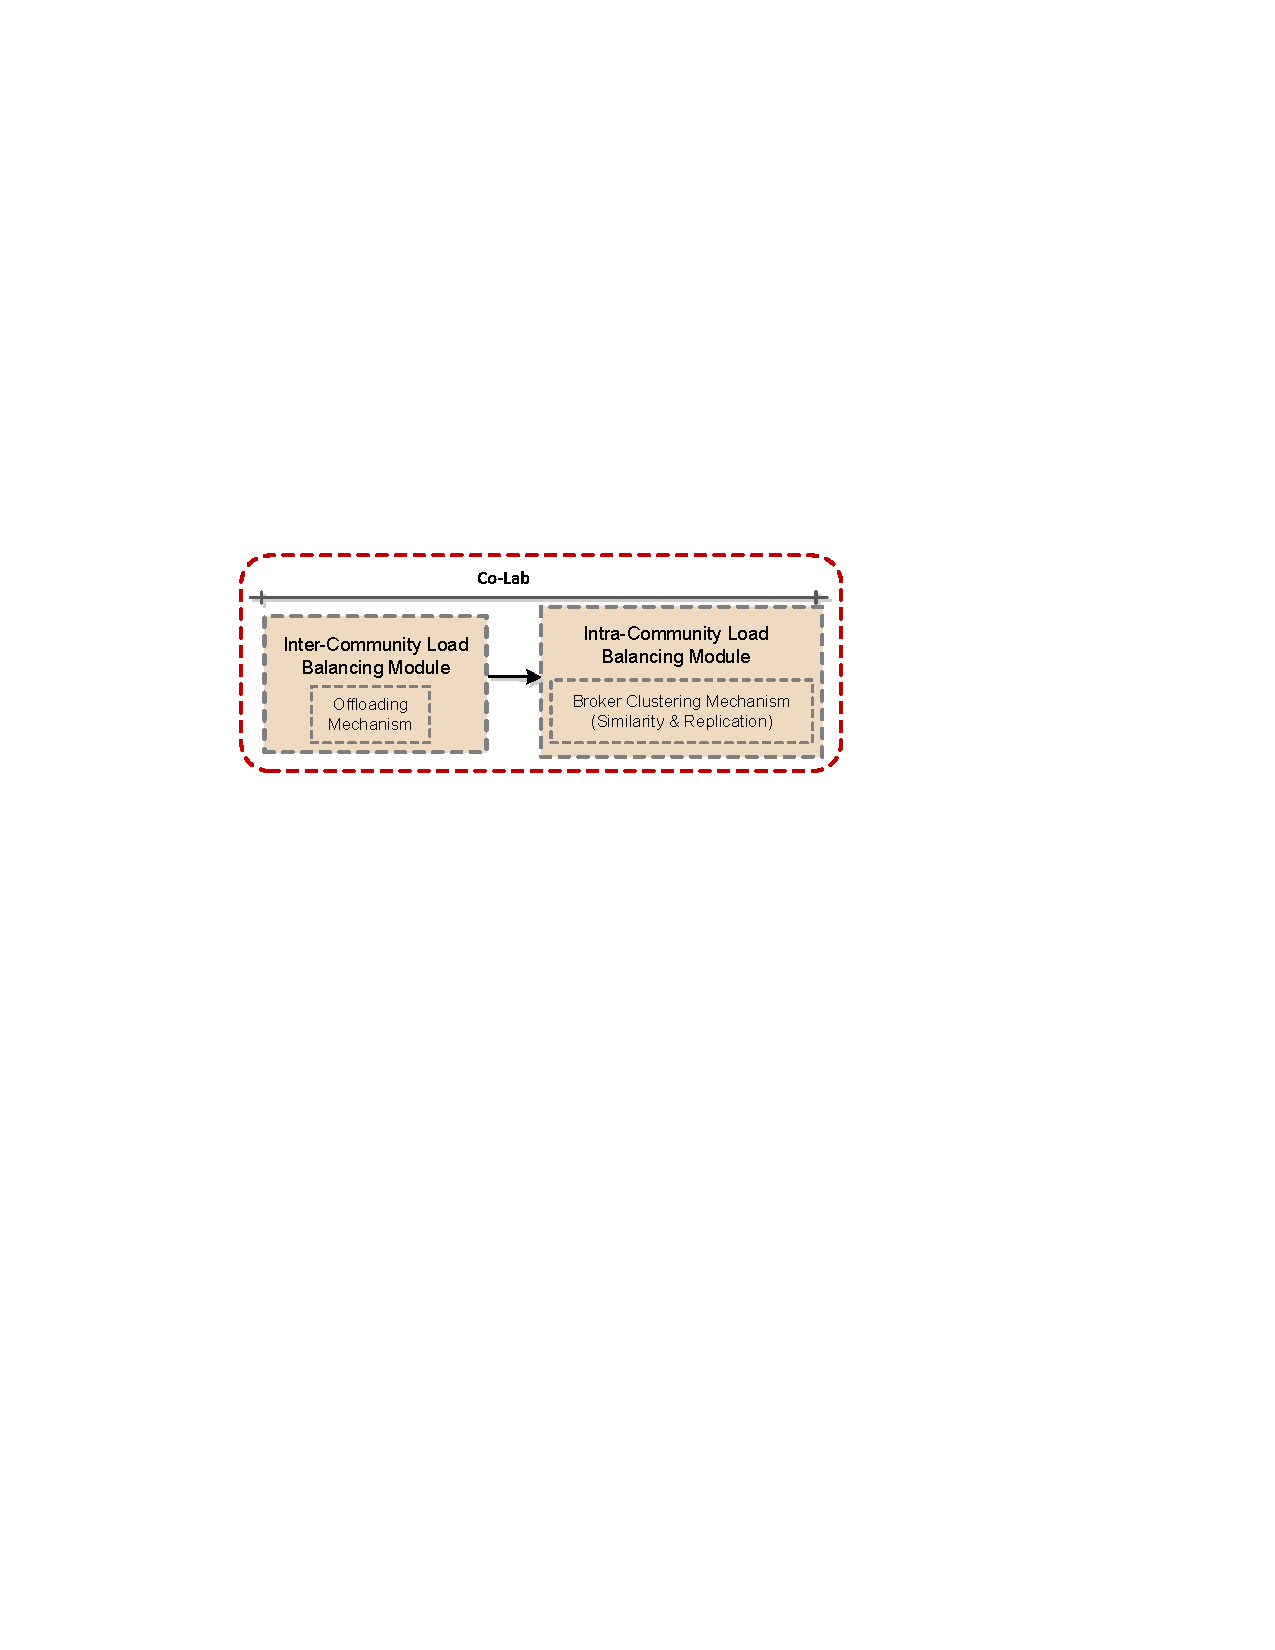
\includegraphics[width=0.68\textwidth]{Chap5-Fig4.pdf}
  \end{tabular}
  \caption{Co-Lab system model.}
\end{center}
\end{figure}

\subsection{Balancing Inter-Community Load}\label{Chap5_04_01}
\esubsection{Balancing Inter-Community Load}
When a broker $B_i$ is overloaded, the first step it takes to balance its load is by invoking the inter-community load balancing module. In this case, if the broker is receiving publications and subscriptions of events more than its capacity, the inter-community load balancing module decreases the broker's load by offloading the extra inter-community event dissemination load to other brokers in its community that have inter-community links/friendships with under-loaded brokers. Brokers in the same community can balance their load by invoking the similarity-based intra-community load balancing module as discussed in the following sub-section (5.4.2).

After finding the under-loaded broker, a portion of the load is sent to this broker to be processed at the intra-community level. The receiving broker treats these incoming events as the content that is received by itself and initiates a broker clustering phase. It is also possible that some of the brokers become overloaded and do not accept the incoming publications from other community. In this case, the publisher finds an under-loaded broker in its community as described above. Note that broker clustering and filter replication based on similarity are not applicable for the inter-community load balancing mechanism. The inter-community load balancing operation has two cases:
\begin{enumerate}
  \item[$\ast$]Case 1 - All the brokers in the publishers inter-community link ($A_{InterCom}$) are overloaded: the publisher broker ($B_A$) searches a broker $B_h$ in its own community which has an under-loaded inter-community link and then $B_A$ forwards the publication to $B_h$. If all the brokers ($B_i$) in $B_h$'s inter-community link are also overloaded, then $B_h$ search for a broker $B_k$ in the same community and deliver the event to $B_i$'s community through $B_k$'s inter-community link. However, if all the brokers $B_i$ in $B_h$'s inter-community link are not overloaded, then $B_h$ directly sends the event to $B_i$.
  \item[$\ast$]Case 2 - All the brokers in $A_{InterCom}$ are not overloaded (under-loaded): $B_A$ sends the event straight to $B_i$.
\end{enumerate}

\subsection{Exploiting Similarity for Intra-Community Load Balancing}\label{Chap5_04_02}
\esubsection{Exploiting Similarity for Intra-Community Load Balancing}

Our proposed filter replication solution ensures that the load of a clustered broker is in the range of [$\BigO{\frac{\ln\ln A_{\theta_G}}{\ln G}} - \BigO1$, $\BigO{\frac{\ln\ln A_{\theta_G}}{\ln G}} + \BigO1$] as shown in the previous section. It's obvious that given a number of brokers in the community, there are exponential possibilities to form clusters among the brokers. In this regard, among the exponential possibilities to make clusters of brokers, we hope that the overall load of the clusters in the community has the possibility to be lesser than the overall loads before the formation of clusters. Therefore, we initially start by exploiting similarity for clustering brokers as follows.

The minimum load among the non-clustered brokers before replication is $A_{\theta_i}$, where $\theta_i$ represents the list of filters on a particular broker $B_i$ having the load $A_{\theta_i}$. On the other hand, the maximum load inside the $G$ clustered brokers after replication is $\BigO{\frac{\ln\ln A_{\theta_G}}{\ln G}} + \BigO1$. Therefore, it is possible to conclude that clustered brokers have less load than the non-clustered brokers in the community, if the following condition satisfies.
\begin{equation}
\BigO{\frac{\ln\ln A_{\theta_G}}{\ln G}} + \BigO1 \leq A_{\theta_i}.
\end{equation}

Before we describe how to formulate and compute the similarity between filters in detail, we first give an illustration of greedy forwarding approach for checking how Equation 5.6 can be satisfied. Consider two brokers $B_1$ and $B_2$ have filters $\theta_1$ and $\theta_2$ respectively, and receive total publications of $A_{\theta_1} + A_{\theta_2} = 30$ before replication. Then, we cluster the two brokers and replicate the filters ($\theta_1 \cup \theta_2$) onto both $B_1$ and $B_2$. Our goal here is to measure the load of the clustered brokers $B_1$ and $B_2$ after the adoption of greedy forwarding approach. As shown in Table 5.1, we use five different examples for specific $\theta_1$, $\theta_2$, $A_{\theta_1}$ and $A_{\theta_2}$.

\begin{table}\fontsize{8.6}{10}\selectfont
\centering
\caption{Examples of load calculation for brokers $B_1$ and $B_2$ before and after replication}
\renewcommand{\arraystretch}{2.3}
\begin{tabular}{|c|c|c|c|c|c|c|}
\hline
\multicolumn{1}{c}{{Ex.}} & \multicolumn{1}{c}{{Similarity}} & \multicolumn{1}{c}{{$A_{\theta_1}$ [BR]}} & \multicolumn{1}{c}{{$A_{\theta_2}$ [BR]}} & \multicolumn{1}{c}{{$A_{\theta_1}$ [AR]}} & \multicolumn{1}{c}{{$A_{\theta_2}$ [AR]}} &
\multicolumn{1}{c}{{Remark}}\\
\hline
\multicolumn{1}{c}{1} & \multicolumn{1}{c}{$A_{\theta_1} \cap A_{\theta_2}=0$} & \multicolumn{1}{c}{$A_{\theta_1}=29$} & \multicolumn{1}{c}{$A_{\theta_2}=1$} & \multicolumn{1}{c}{$A_{\theta_1}=15$} & \multicolumn{1}{c}{$A_{\theta_2}=15$} & \multicolumn{1}{c}{15>1, this indicates AR incurs heavier load for $B_2$}\\
\multicolumn{1}{c}{2} & \multicolumn{1}{c}{$A_{\theta_1} \cap A_{\theta_2}=4$} & \multicolumn{1}{c}{$A_{\theta_1}=25$} & \multicolumn{1}{c}{$A_{\theta_2}=5$} & \multicolumn{1}{c}{$A_{\theta_1}=13$} & \multicolumn{1}{c}{$A_{\theta_2}=13$} & \multicolumn{1}{c}{13>5, this shows AR incurs slightly heavier load for $B_2$}\\
\multicolumn{1}{c}{3} & \multicolumn{1}{c}{$A_{\theta_1} \cap A_{\theta_2}=5$} & \multicolumn{1}{c}{$A_{\theta_1}=20$} & \multicolumn{1}{c}{$A_{\theta_2}=10$} & \multicolumn{1}{c}{$A_{\theta_1}=13$} & \multicolumn{1}{c}{$A_{\theta_2}=12$} & \multicolumn{1}{c}{12>10, AR incurs very few heavier load for $B_2$}\\
\multicolumn{1}{c}{4} & \multicolumn{1}{c}{$A_{\theta_1} \cap A_{\theta_2}=10$} & \multicolumn{1}{c}{$A_{\theta_1}=15$} & \multicolumn{1}{c}{$A_{\theta_2}=15$} & \multicolumn{1}{c}{$A_{\theta_1}=10$} & \multicolumn{1}{c}{$A_{\theta_2}=10$} & \multicolumn{1}{c}{10<15, AR leads to lighter load for both $B_1$ \& $B_2$}\\
\multicolumn{1}{c}{5} & \multicolumn{1}{c}{$A_{\theta_1} \cap A_{\theta_2}=15$} & \multicolumn{1}{c}{$A_{\theta_1}=15$} & \multicolumn{1}{c}{$A_{\theta_2}=15$} & \multicolumn{1}{c}{$A_{\theta_1}=8$} & \multicolumn{1}{c}{$A_{\theta_2}=7$} & \multicolumn{1}{c}{7<15, AR leads to balanced load for both $B_1$ \& $B_2$}\\
\hline
\multicolumn{7}{c}{(BR and AR denotes before and after replication, respectively)}\\
\end{tabular}
\end{table}

As shown in Table 5.1 that provides examples, we found out that given the similarity of filters (i.e. $\theta_1 = \theta_2$ or $\theta_1 \approx \theta_2$ in the fourth and fifth examples), the condition in Equation 5.6 satisfies. For instance, in Ex. 1 where there is no interest similarity between the events matching $\theta_1$ and $\theta_2$ ($A_{\theta_1} \cap A_{\theta_2}=0$), the replication operation incurs heavier load for $B_2$ (from one events matching this broker to 15 events). Therefore, the most valuable criterion to decide whether or not two brokers can form a cluster becomes the similarity between the corresponding filters.
\begin{equation}
Sim(B_1, B_2)=Sim(\theta_1, \theta_2)=Sim(A_{\theta_1}, A_{\theta_2}).
\end{equation}

To compute the similarity between the two filters ($Sim(\theta_1, \theta_2)$), we choose to consider the publications that match $\theta_1 \cap \theta_2$ and $\theta_1 \cup \theta_2$. Based on this logic, we measure the similarity between two brokers $B_1$ and $B_2$ as follows.
\begin{equation}
Sim(\theta_1, \theta_2)=\frac{A_{\theta_1} \cap A_{\theta_2}}{A_{\theta_1} \cup A_{\theta_2}}.
\end{equation}

The two formulas above (i.e. Equations 5.7 and 5.8) cover both the filters and publications matching the filters. In the remaining part of this section, we would like to cluster brokers having high similarity within the community based on the defined similarity metrics as shown in Algorithm 4.

\begin{algorithm}
  \Begin{
     Create and initiate a temporary storage $\chi$, and a list $\nu$ to contain set of clusters of brokers\;
     \For{pair of brokers $B_i$ and $B_j$}{
         store $Sim(B_i, B_j)$ together with $[B_i, B_j]$ to $\chi$;
     }
     \While {$\chi \neq$ empty}{
         get $[B_i, B_j]$ in descending order of $Sim(B_i, B_j)$ (highest similarity first)\;
         \If {both $B_i$ and $B_j$ are already clustered}{
            No action is needed;
         }
        \If{$B_i$ or $B_j$ (i.e. $B_j$) is already in cluster $G_1$}{
            \If {adding $B_i$ to $G_1$ satisfies Equation 5.6}{
                add $B_i$ to $G_1$;}
            \Else
                {start a new cluster $G_2$, add $B_i$ to it, and add $G_2$ to $\nu$;}
            }
        \Else (//both $B_i$ and $B_j$ are not clustered)
                {start a new cluster $G_2$, add both $B_1$ and $B_2$ to it, and add $G_2$ to $\nu$;
        }
        Temporary storage $\chi$ is empty
     }
     \For{$G \in \nu$}{
        replicate filters and create links among member brokers in $G$;
     }
}
\caption{Pseudocode of broker clustering}
\label{alg:chap5_alg02}
\end{algorithm}

\section{Evaluation}\label{Chap5_05}
\esection{Evaluation}
In this section, we evaluate the performance of our proposed load balancing scheme Co-Lab, by comparing it with the method (we call it Offloading) proposed by Cheung and Jacobse~\cite{AKYCheung2010}, Shuffle~\cite{HZhang2008}, and event dissemination algorithm with no particular load balancing approach (we name it as No Load Balancing). One of the main challenges we faced in evaluating our approach is the lack of real world application datasets. However, it is possible to create and generate a topology that mimics the structure of social graph for publish/subscribe network systems. Therefore, we used our own social graph applied in chapter~\ref{Chap4} (ComPAS). The generated graph has 1200 nodes, 17900 number of links/edges with average degree of 15. Communities are structured based on the method presented in sub-section~\ref{Chap5_03_01}. We then randomly chose nodes in the community as brokers, publishers and subscribers.

The matching ratio $\ell$ (ranging from 0 to 100\%) was used to generate filters and publications. Using wide variety of $\ell$ in our evaluation, the results can be interpreted for both Zipf and unform distributions. The parameter range for number of brokers, publishers and subscribers is 0-500, 0-50 and 0-250, respectively. By varying the number of these parameters we conducted the evaluation. As a default, we used 500 broker, 50 publisher and 250 subscriber nodes. The normal distribution is represented by 0.5$\ell$, where the probability of subscriptions is almost equal for all events. High (>50$\ell$) and low (<50$\ell$) implies Zipf distribution where some events are very popular and have many subscribers while other events are very selective and a small number of brokers have subscriptions for these events. The performance of Co-Lab has been analyzed and compared with Offloading, Shuffle, and No Load Balancing in terms of the metrics collected for our analysis as mentioned below.

\subsection{Event Dissemination Load Distribution}\label{Chap5_05_01}
\esubsection{Event Dissemination Load Distribution}
\begin{figure}[t]
\begin{center}
  \begin{tabular}{c}
  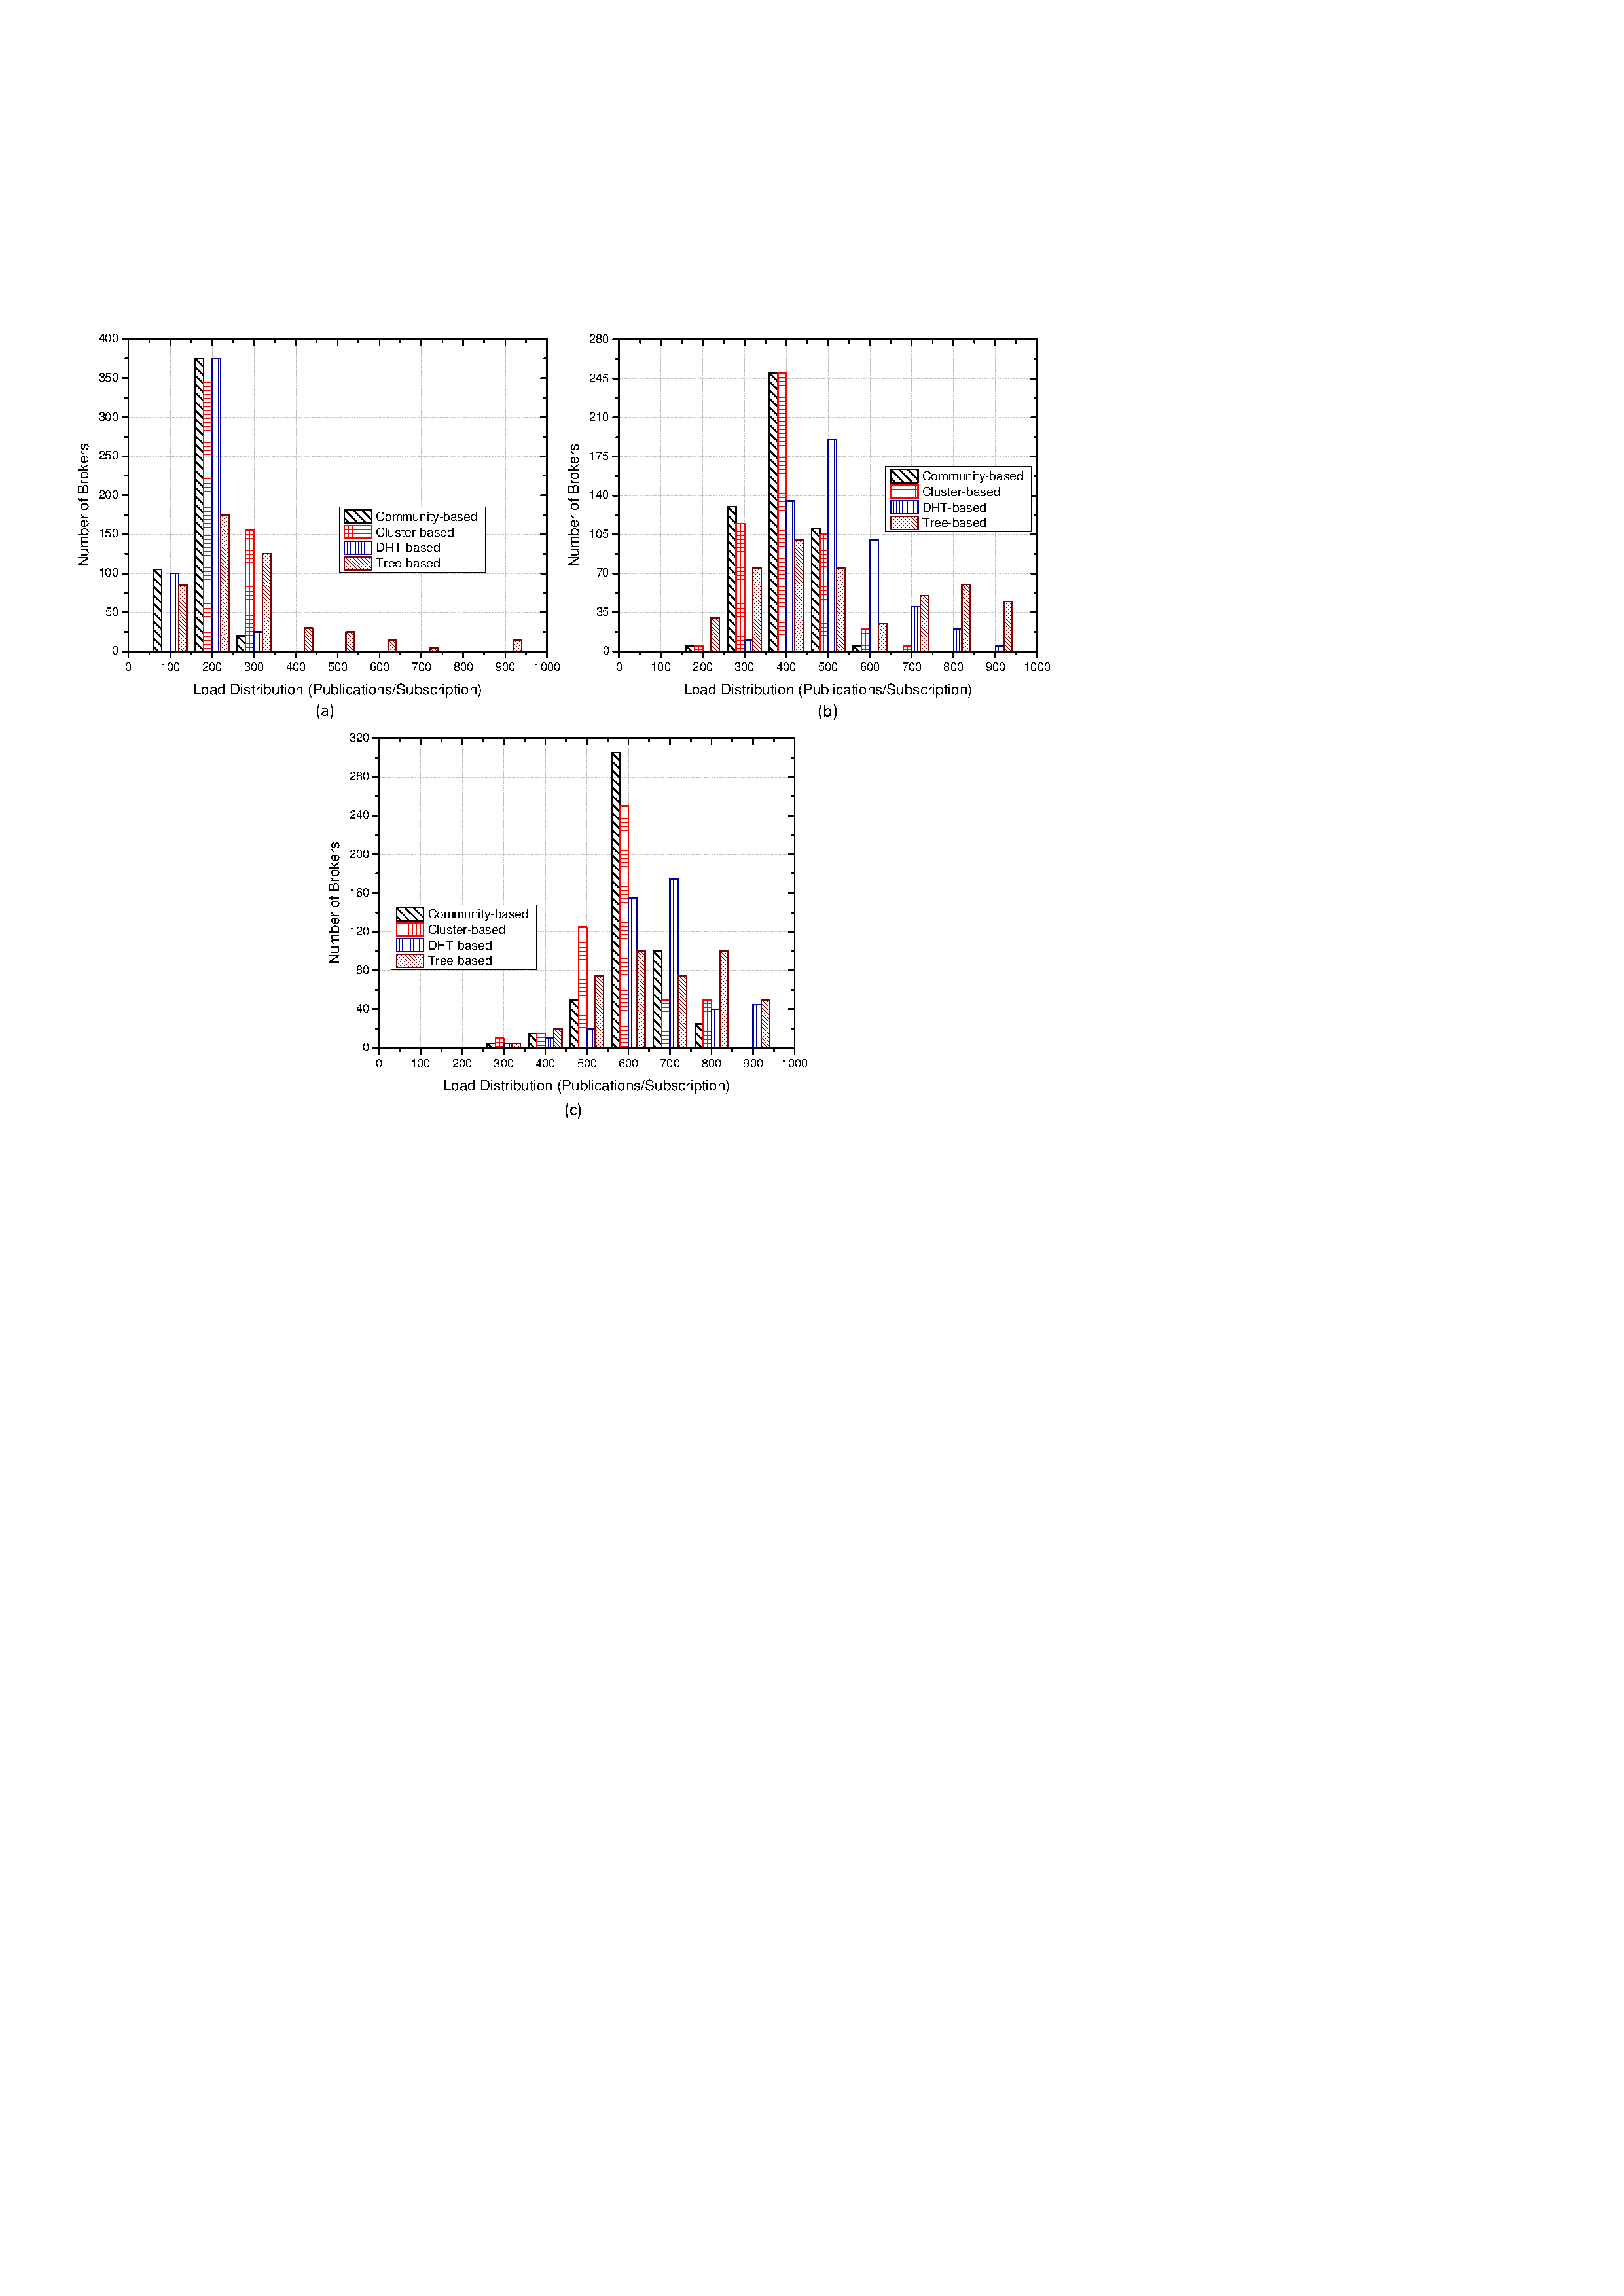
\includegraphics[width=0.95\textwidth]{Chap5-Ev-Fig1a.pdf}
  \end{tabular}
  \caption{Load distribution of event dissemination for Community-based, Cluster-based, DHT-based and Tree-based approaches based on (a) 0.25$\ell$, (b) 0.5$\ell$, (c) 0.75$\ell$.}
\end{center}
\end{figure}

As depicted in Figs. 5.5(a)-(c), we first compare our approach (community-based load balancing) with three other common load balancing approaches, tree-based, DHT-based, and cluster-based. The evaluation is based on the number of events that is managed by a broker in one time unit and the publications and subscriptions are uniformly distributed among brokers. Figs. 5.5(a)-(c) presents the dissemination of load distribution for three different matching ratios ($\ell$=0.25, $\ell$=0.5 and $\ell$=0.75). Tree-based approach performs the worst in case of load distribution. In all the denoted matching ratios, there are several brokers with very high amounts of load, while there are brokers with very small amounts of load. This can be reasonable based on the tree structure of the broker where any publication from one side that has matching subscription on the other side of the tree must pass through the brokers. These brokers are processing almost all the publications which results in high dissemination load. On the other hand, brokers in the edge of the tree do not participate in publication dissemination very often which results in very small load. The DHT-based system performs somewhat better than the tree-based one, and cluster-based performs better than both tree-based and DHT-based. However, in all cases our community-based load balancing method, disseminates the load more consistently and uniformly among brokers and circumvent highly overloaded brokers.

\begin{figure}[t]
\begin{center}
  \begin{tabular}{c}
  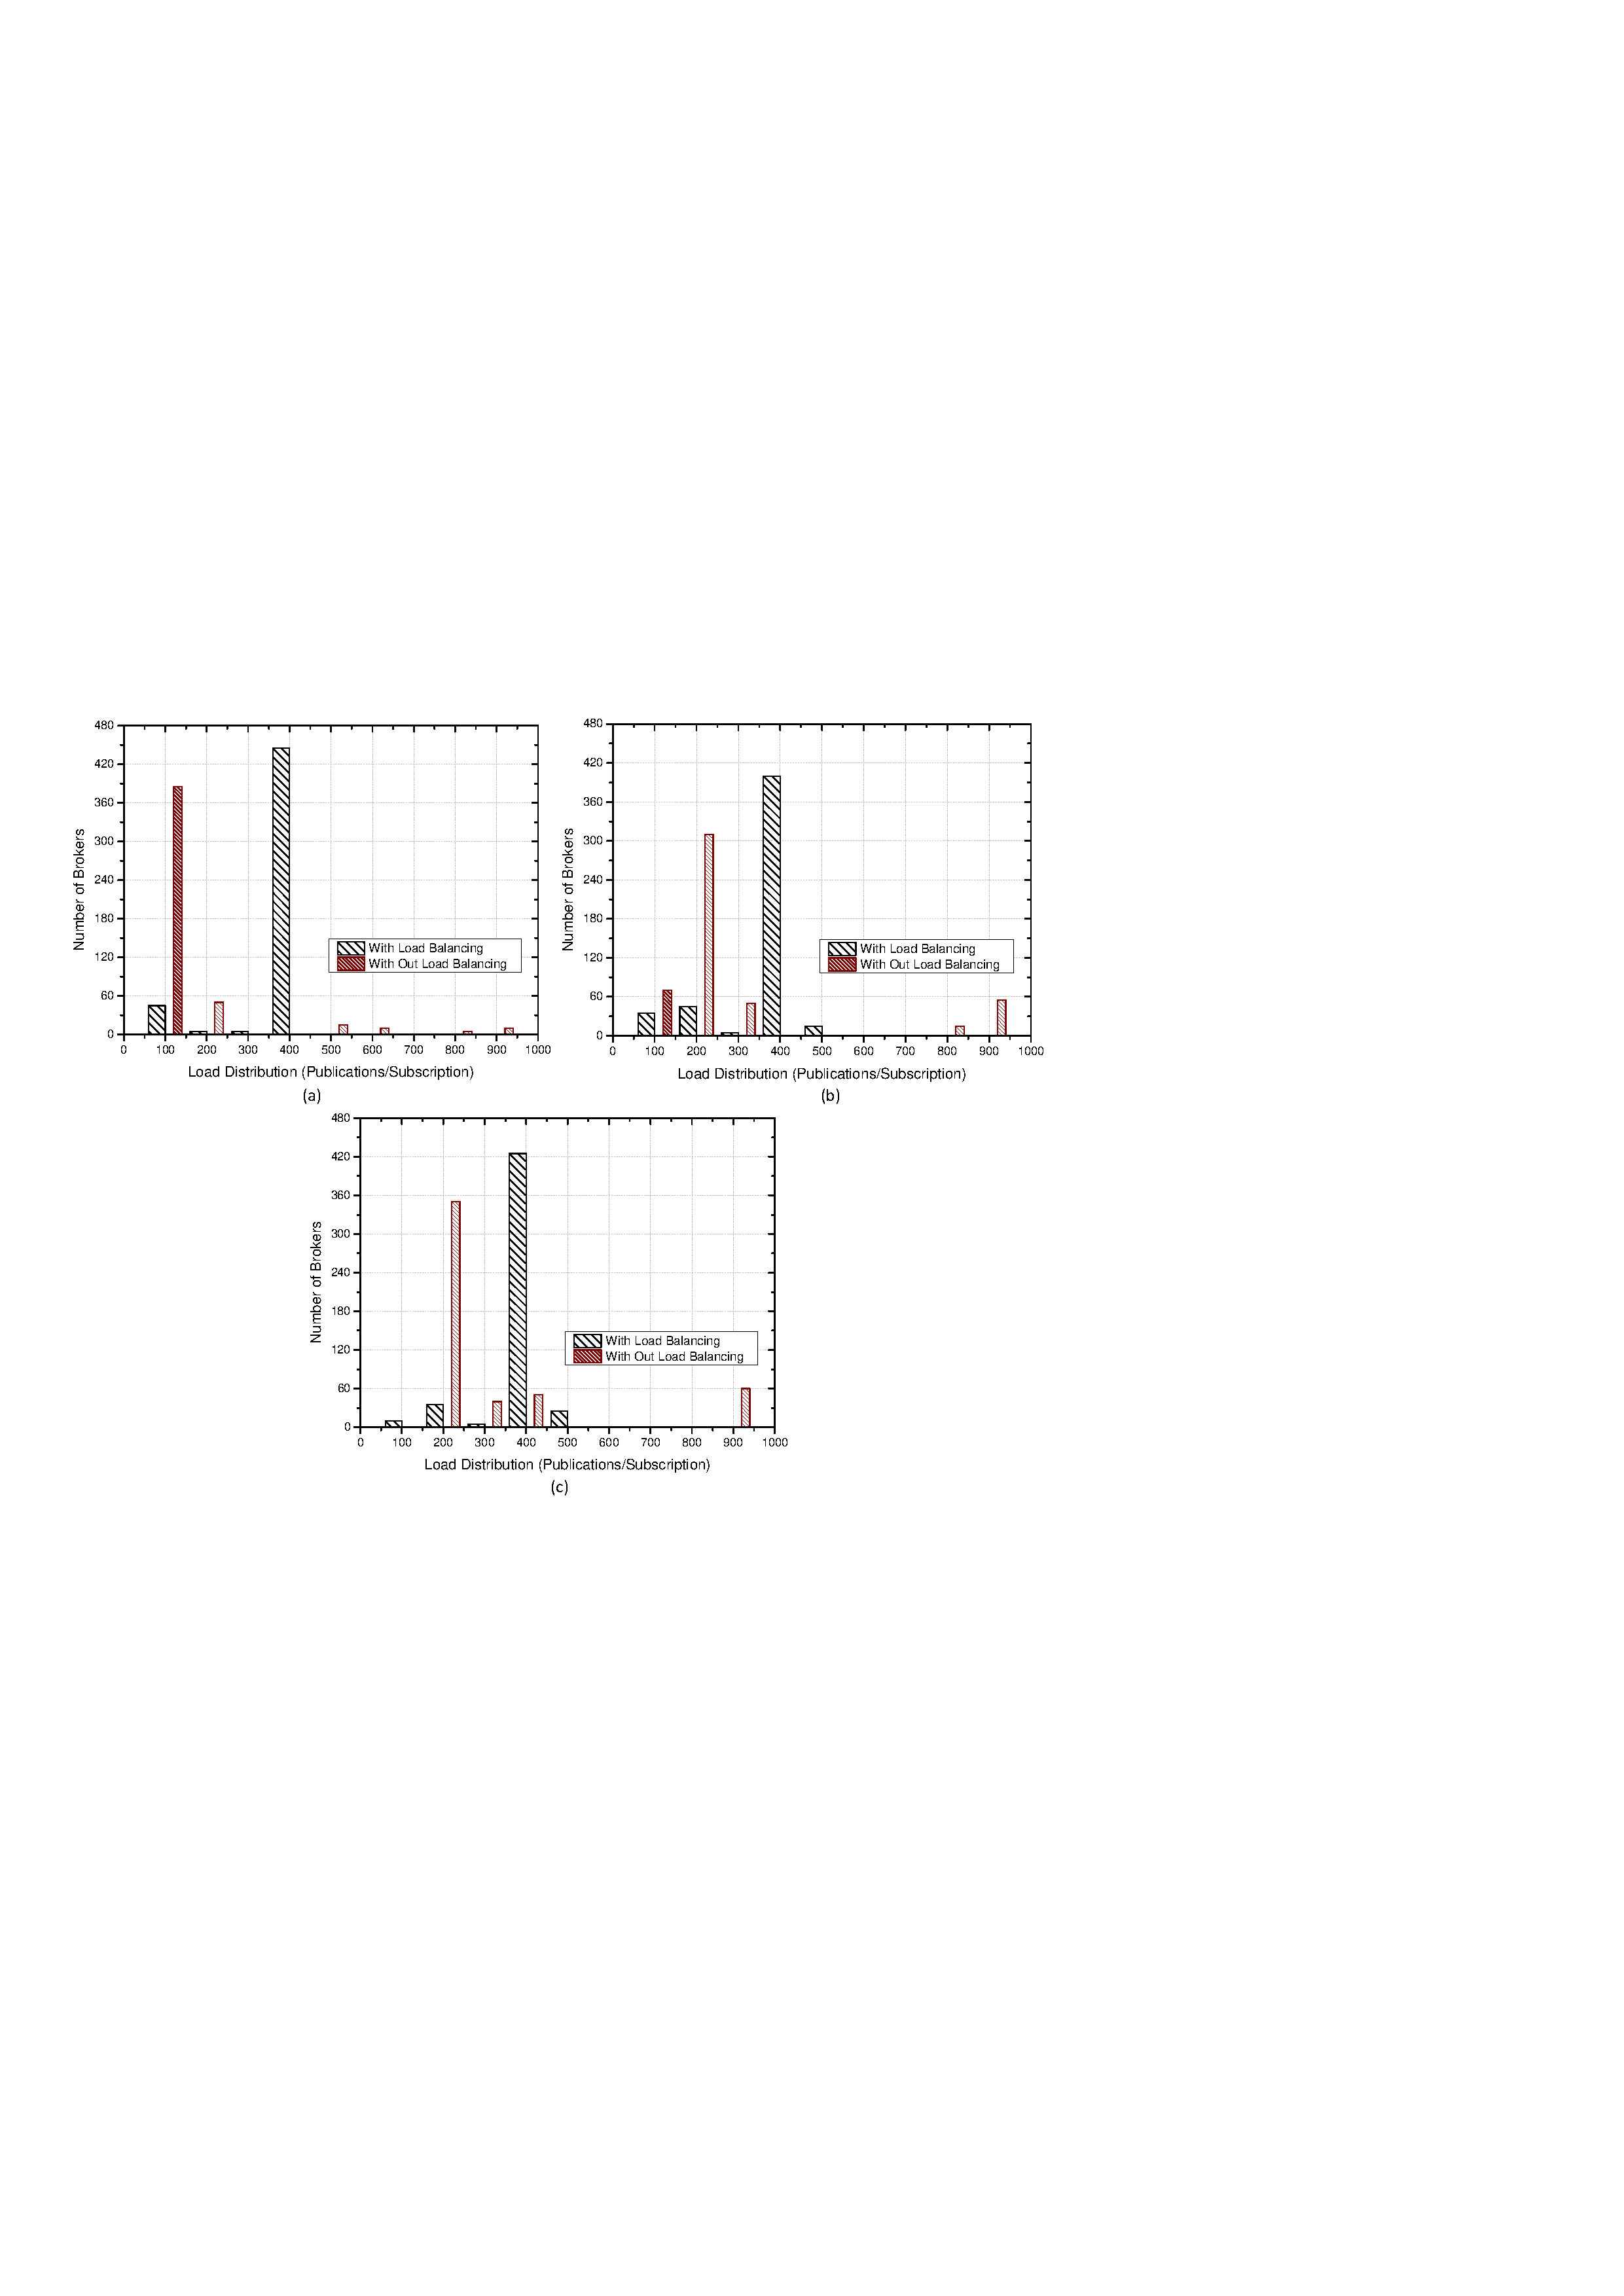
\includegraphics[width=0.95\textwidth]{Chap5-Ev-Fig1b.pdf}
  \end{tabular}
  \caption{Community-based event dissemination with and without load balancing mechanism based on (a) 0.25$\ell$, (b) 0.5$\ell$, (c) 0.75$\ell$.}
\end{center}
\end{figure}

In Figs. 5.6(a)-(c), we present the evaluation of the proposed community-based technique with and without load balancing in order to show the significance of the load balancing algorithm. Our method is compared with the other using three different matching ratios, 25\% ($\ell$=0.25), 50\% ($\ell$=0.5) and 75\% ($\ell$=0.75). The plots clearly show that when the publication distribution among brokers follows Zipf distribution (for $\ell$=0.25 and $\ell$=0.75), the community-based approach without load balancing results in irregular or uneven distribution of dissemination load. This is because of concentration of dissemination load on a small portion of inter-community in the network which results in higher dissemination load on the brokers while the other brokers in the other communities remain under-loaded. Contrarily, in community-based event dissemination with load balancing, brokers at the inter-community link with higher load offloads some of the load to brokers in the other community link with smaller load which results in more uniform distribution of load among brokers. As seen in Fig. 5.6(a), regarding community-based with load balancing, almost 90\% of brokers have a load in range [300, 400] and there is no broker with higher load. However, the same plot with no load balancing technique shows that the load distribution is very skewed and more than 70\% of brokers have a load in range [0, 100] while around 15\% of brokers have a load higher than 500. The same results are obtained for $\ell$=0.5 and $\ell$=0.75 which validates our load balancing method in efficiently balancing the load among brokers and preventing broker overloading as much as possible.

\subsection{Overall Load}\label{Chap5_05_02}
\esubsection{Overall Load}
To evaluate the overall load, we specify and amount the overall publications received by all brokers in the community. As depicted in Fig. 5.7(a), as the number of brokers increases it incur heavier overall loads for all the load balancing approaches (Co-Lab, Offloading, Shuffle and No Load Balancing). The logic behind this is that, when more brokers are employed on the generated social graph, the subscription clients are more distinctly distributed to the brokers. Therefore, publications are forwarded towards more number of brokers until the publications are received by the last subscribers in the community. The total number of publications are then increased. However, it is noted from the figure that, the average number of event publication per broker becomes smaller. For instance, when the number of brokers grows from 250 to 500, the overall load of our proposed approach, Offloading, Shuffle, and No Load Balancing are increased by 20\%, 22.23\%, 31.67\%, and 30.26\% respectively, while the average publication per broker is decreased by 37.5\%, 35.71\%, 26.83\%, and 28.3\%.
\begin{figure}[t]
\begin{center}
  \begin{tabular}{c}
  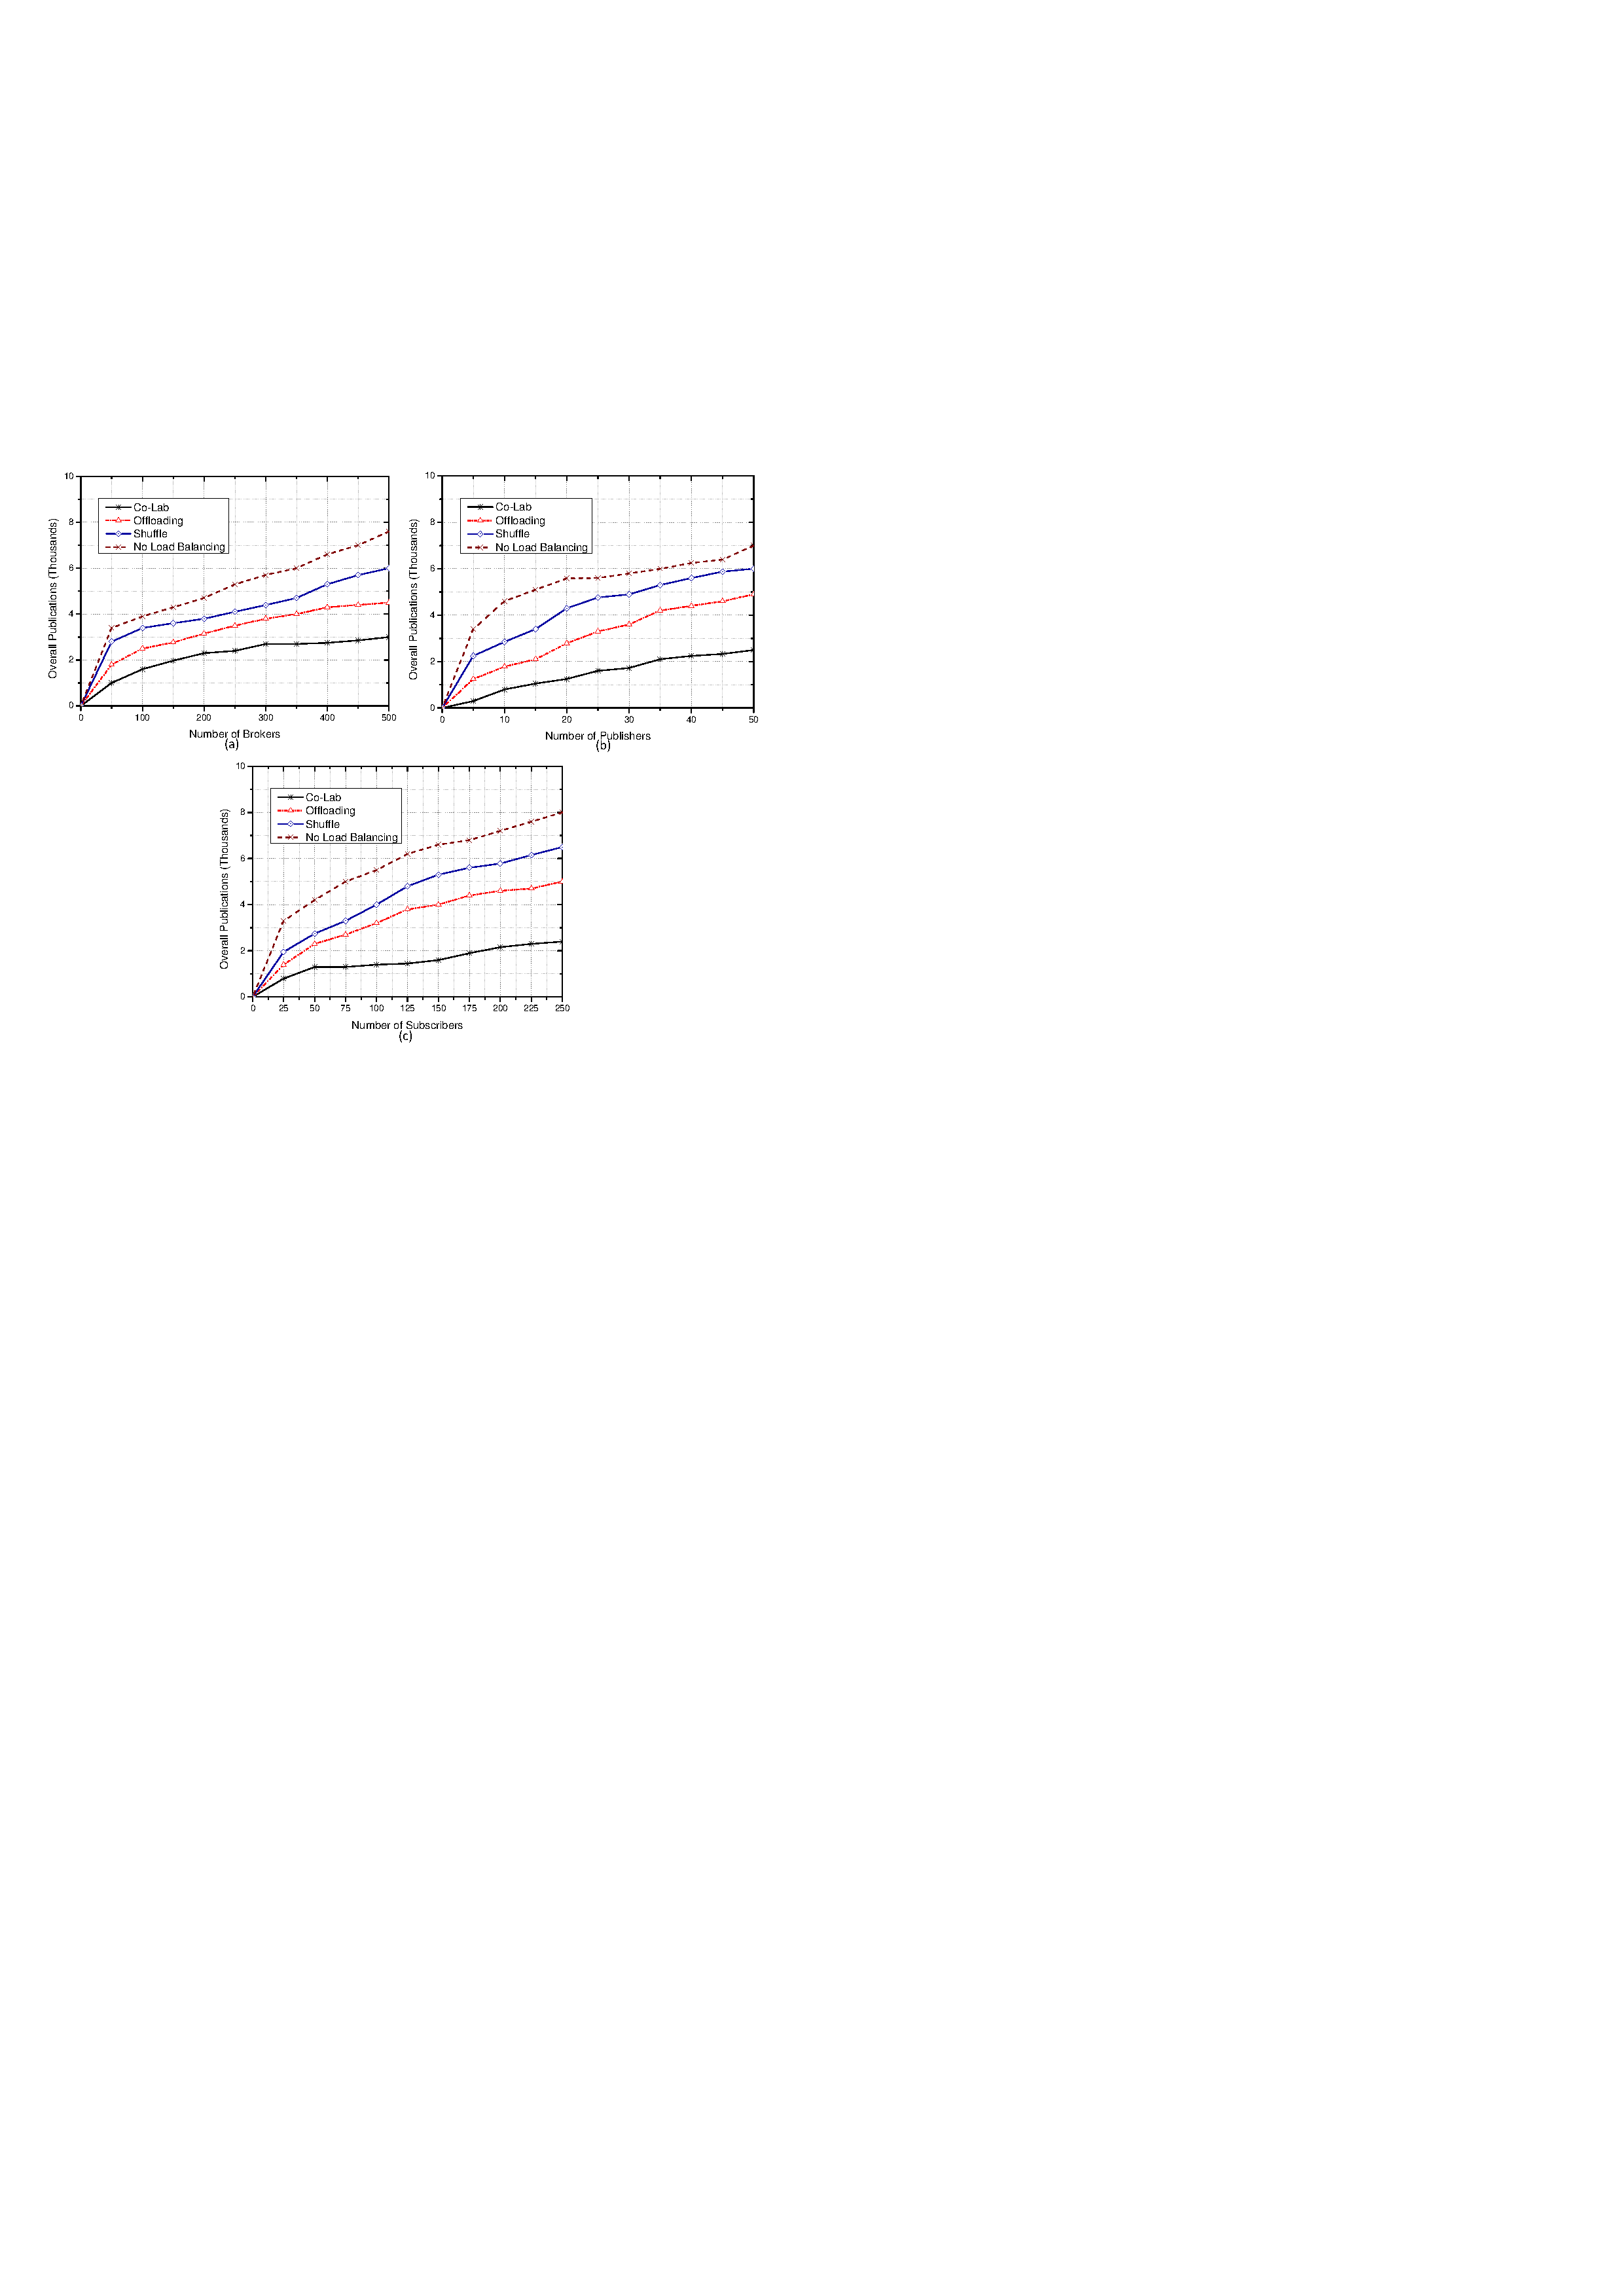
\includegraphics[width=0.95\textwidth]{Chap5-Ev-Fig2.pdf}
  \end{tabular}
  \caption{Overall workloads of all brokers in the communities based on the effect of (a) brokers, (b) publishers, and (c) subscribers.}
\end{center}
\end{figure}

Fig. 5.7(b) displays, when the number of publishers increases the system generates more publications, resulting in heavier loads for all the approaches including ours. However, Co-Lab has fewer overall loads than the other three methods. For instance, when the numbers of publishers are at the maximum, which is 50, compared with Offloading, Shuffle, and No Load Balancing, our proposed method achieves 48.98\%, 58.33\%, and 64.29\% reductions of the overall load respectively. Furthermore, the increase in number of subscribers results in heavier overall load for all the approaches; Co-Lab, Offloading, Shuffle, and No Load Balancing. The fact is that, when we balance the number of publishers and the overall generated events, the publications have to be forwarded to more subscribers with a consistently large number of publications, which results in heavier loads as depicted in Fig. 5.7(c). For instance, when the numbers of subscribers are at the maximum, which is 250, compared with Offloading, Shuffle, and No Load Balancing, our proposed method achieves 52\%, 63.02\%, and 70\% reductions of the overall load respectively.

\subsection{Load Distribution}\label{Chap5_05_03}
\esubsection{Load Distribution}
We use a variable $\Omega$ [1, 5] of distribution to measure the load distribution of every broker as displayed in Figs. 5.8(a)-(c). When the $\Omega$ value is higher, there is an even distribution of load among brokers.  As plotted in Fig. 5.8(a), as the numbers of broker increases from 0 to 500, the value of $\Omega$ also increases for all four methods including Co-Lab resulting in a better balanced loads among brokers in the community. When there is large number of brokers, there exist more brokers in the system satisfying the condition of Equation 5.6 to reduce the loads of those overloaded brokers and transfer it to the under-loaded brokers. As a result it achieves better balanced loads of brokers for Co-Lab, Offloading, Shuffle, and No Load Balancing methods.
\begin{figure}[t]
\begin{center}
  \begin{tabular}{c}
  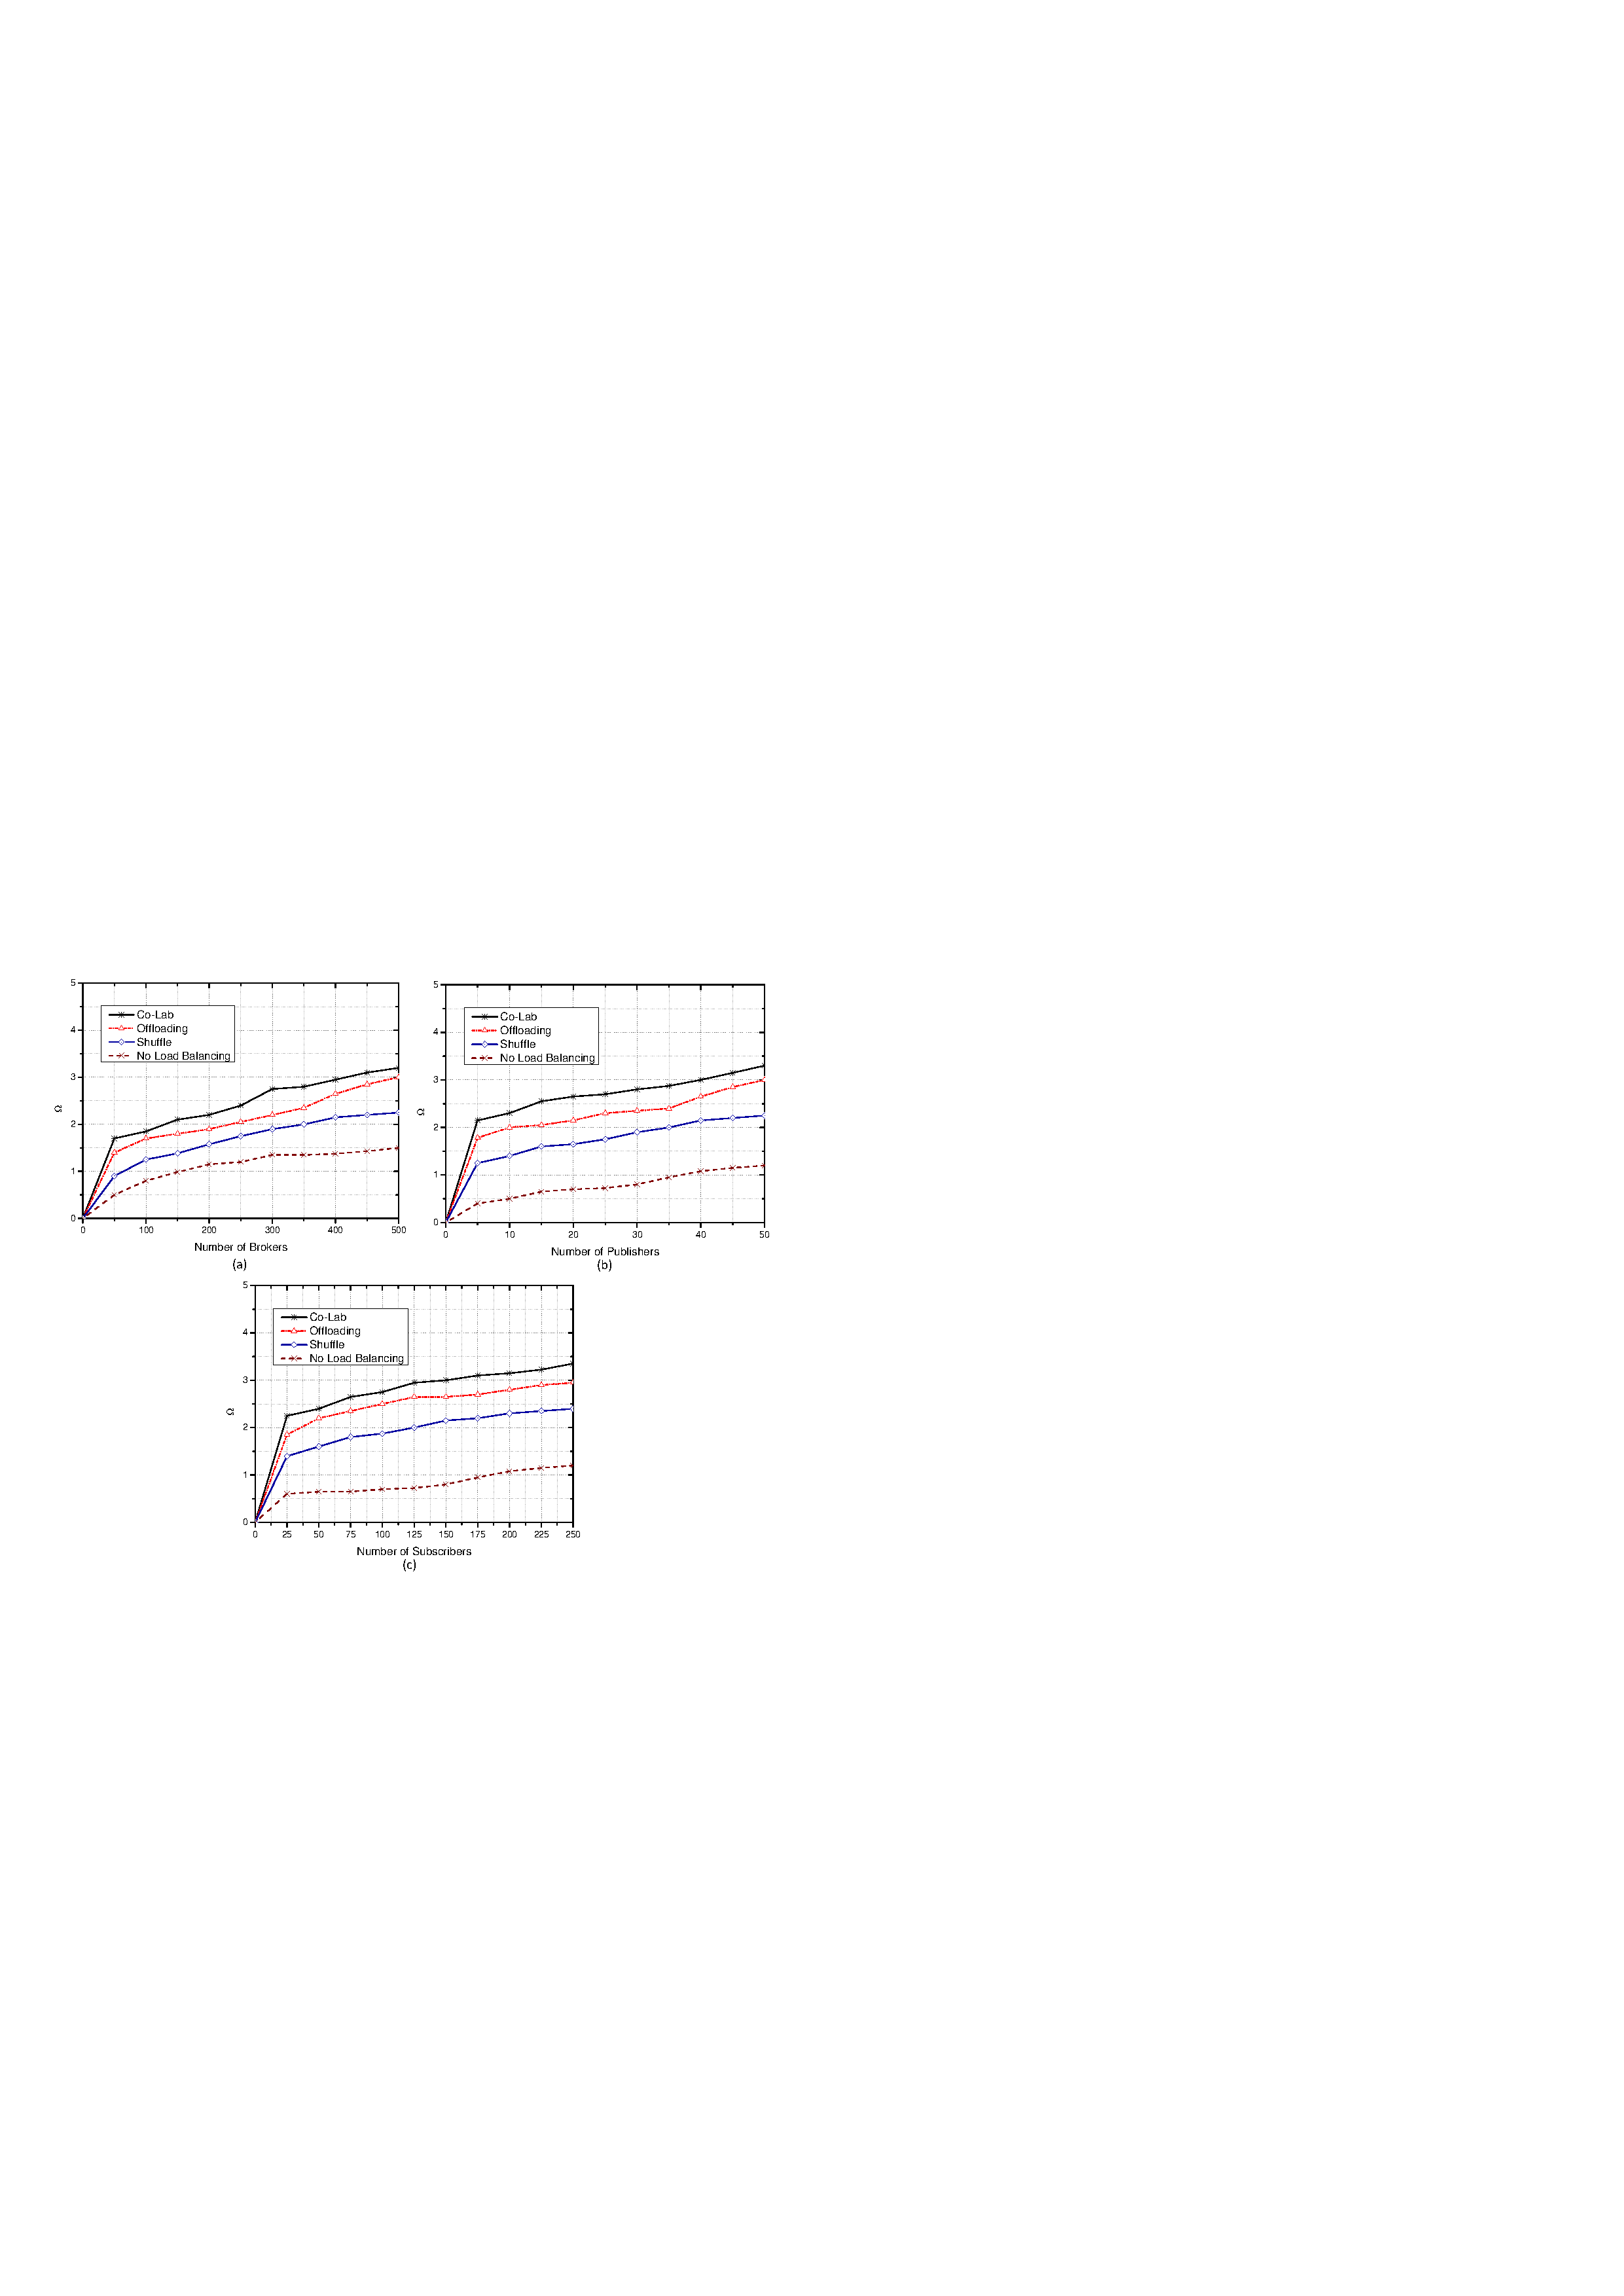
\includegraphics[width=0.95\textwidth]{Chap5-Ev-Fig3.pdf}
  \end{tabular}
  \caption{Load distribution measurement of every broker in their respective communities as influenced by (a) brokers, (b) publishers, and (c) subscribers.}
\end{center}
\end{figure}
\begin{figure}[t]
\begin{center}
  \begin{tabular}{c}
  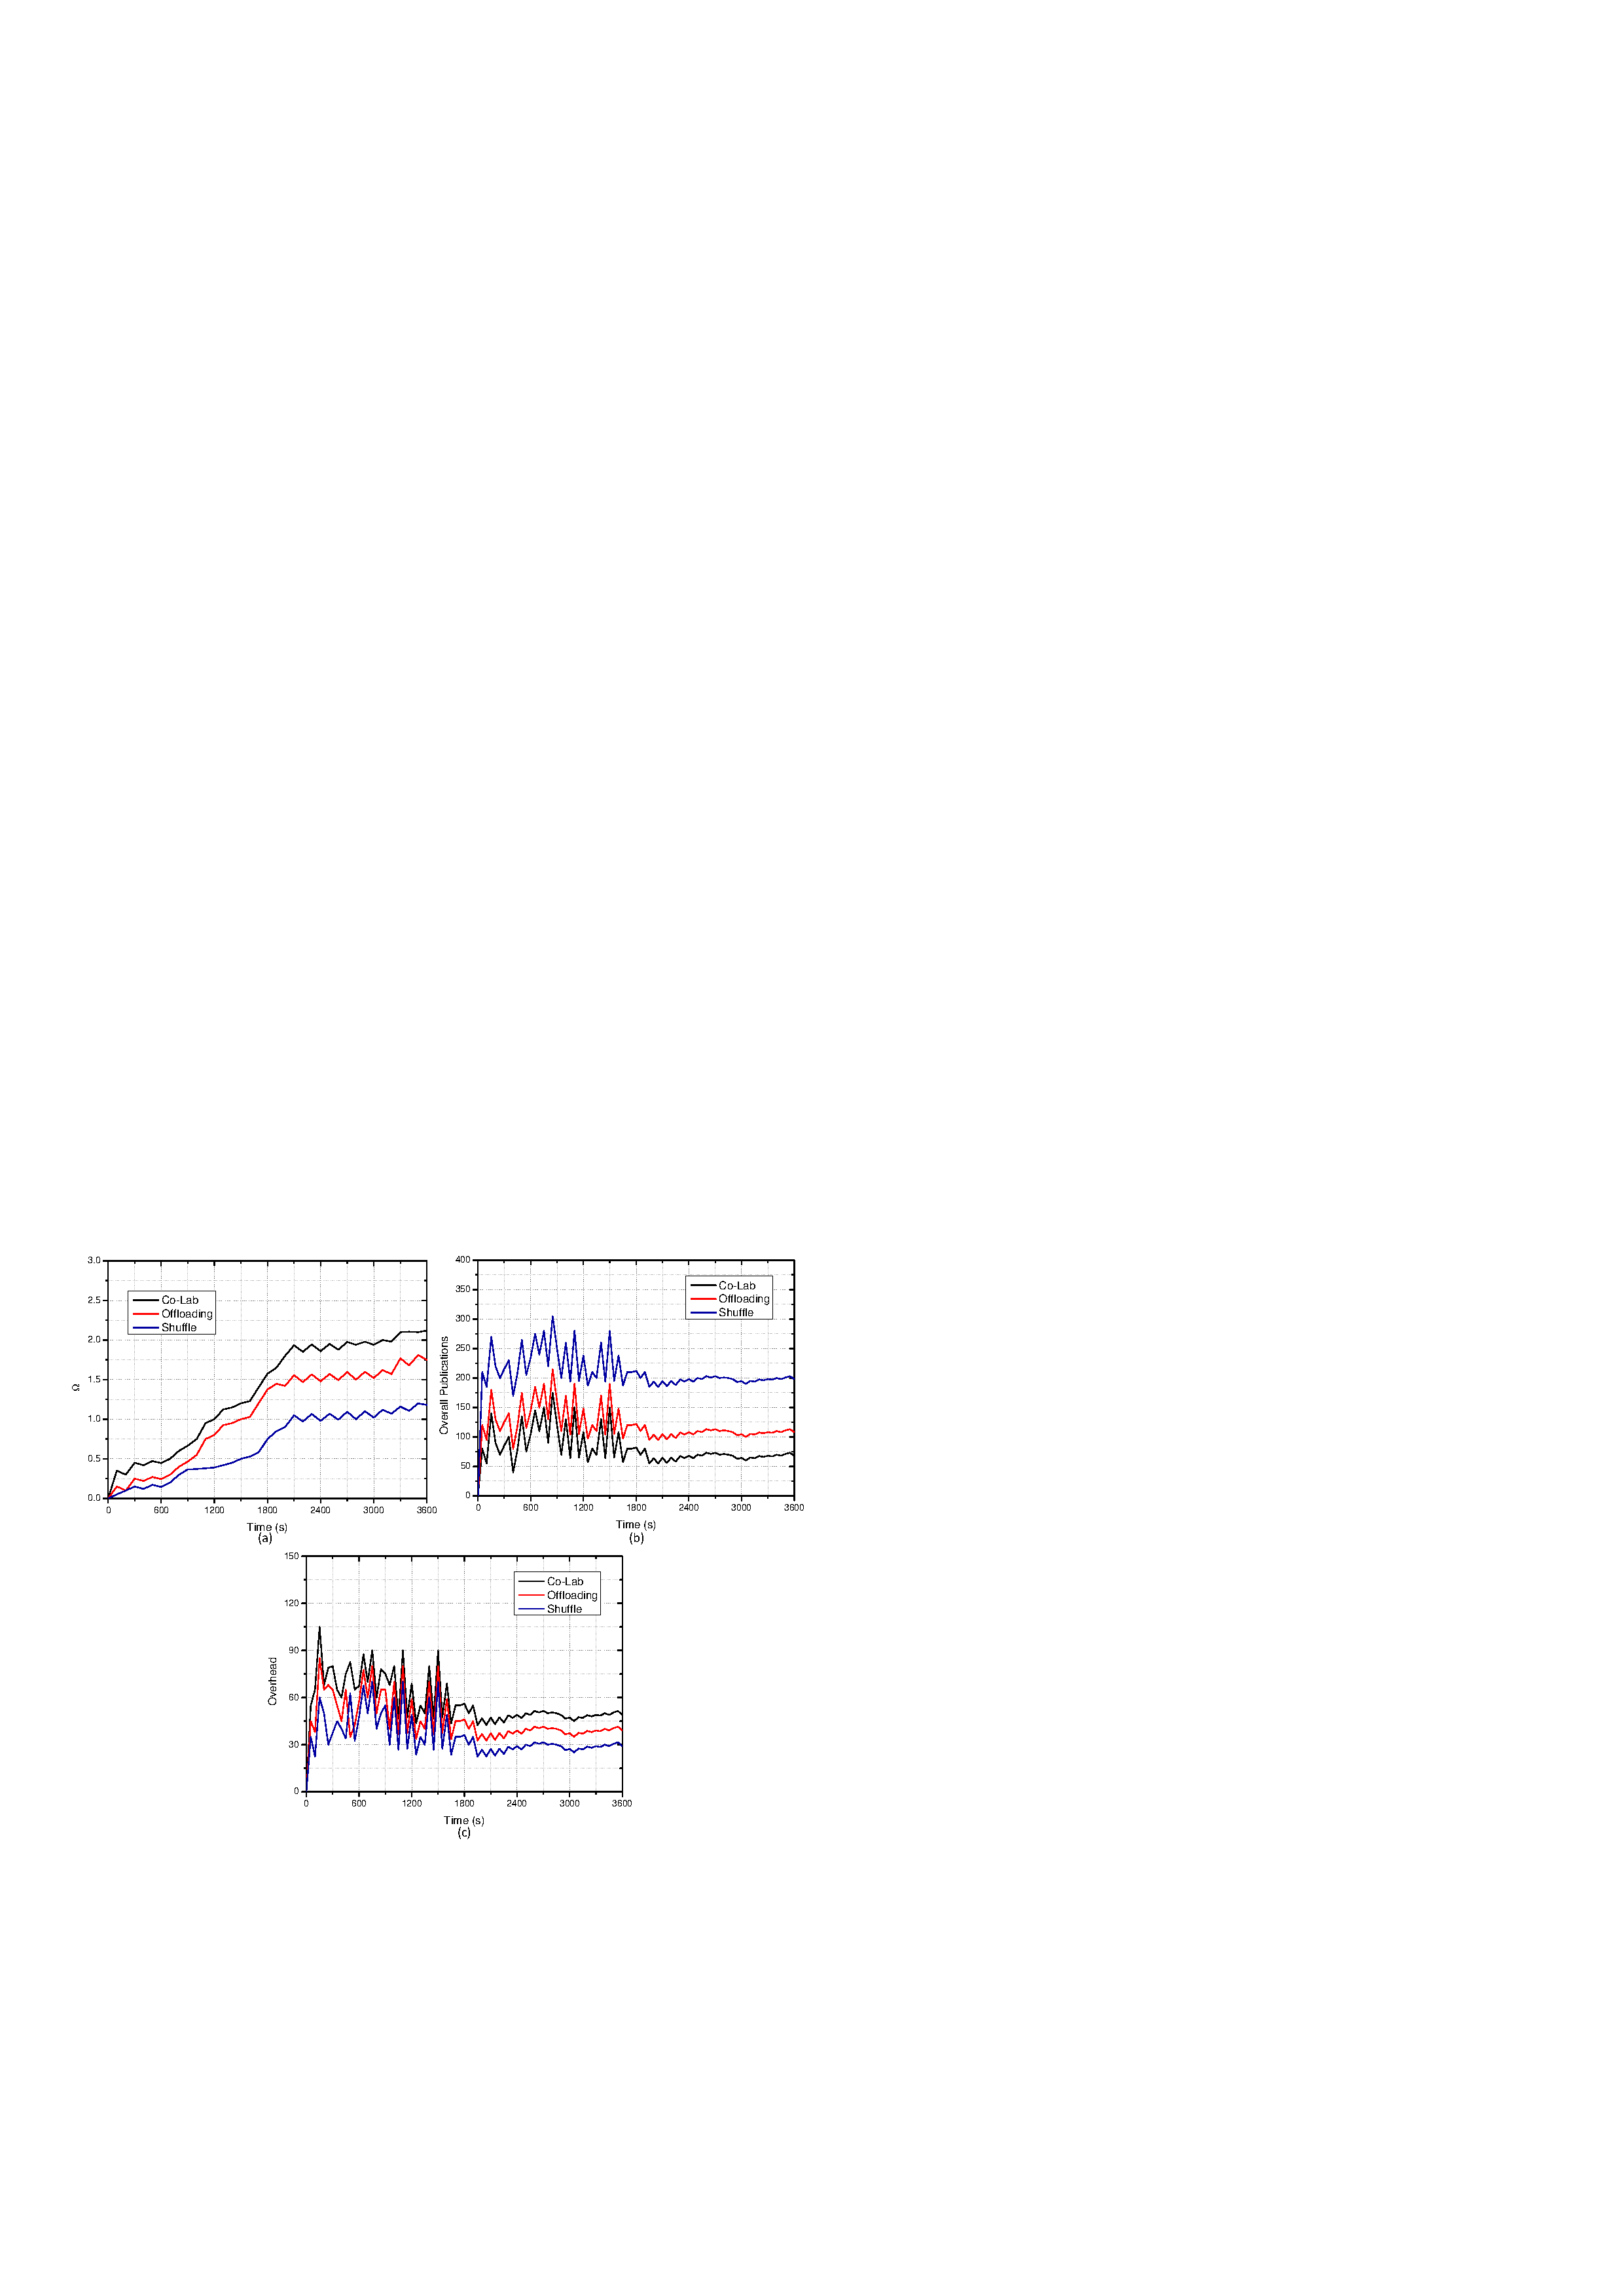
\includegraphics[width=0.95\textwidth]{Chap5-Ev-Fig4.pdf}
  \end{tabular}
  \caption{The effect of varying time on (a) load distribution, (b) overall loads, and (c) overhead of the load balancing methods.}
\end{center}
\end{figure}

In Fig. 5.8(b), we evaluate the effect of number of publishers on the performance of Co-Lab, Offloading, Shuffle, and No Load Balancing. When the number of publishers increases, $\Omega$ value also increases resulting in better balanced load among brokers. Furthermore, as displayed on the figure Co-Lab achieves higher $\Omega$ value than the other three methods. For instance, when the number of publishers reaches the maximum, the $\Omega$ values of Co-Lab, Offloading, Shuffle, and No Load Balancing are 3.3, 3, 2.25, and 1.2 respectively. Moreover, when we vary the number of subscribers from 0 to 250, the $\Omega$ values of all the presented methods grow as shown in Fig. 5.8(c). The reason behind this result is that, more subscribers' results in more subscriptions to the brokers.

\subsection{Load Balancing and Overhead}\label{Chap5_05_04}
\esubsection{Load Balancing and Overhead}

As shown in Figs. 5.9(a)-(c), we investigate the effect of load balancing vary with time on load distribution, overall loads and overhead. We found out that the value of $\Omega$ for all the methods become increasing from the beginning to 2000s and keep on almost the same $\Omega$ value after the moment of 2000 seconds as depicted in Fig. 5.9(a). This implies that the loads are becoming better balanced. Next, we evaluate the overall load distribution by varying the time. As plotted in Fig. 5.9(b), the overall load of all the methods gradually decreases as the time increases. At time 2000s, the overall number of publications of Co-Lab, Offloading, and Shuffle becomes 63.48, 103.54, and 193.46 respectively. Hence, it is obvious to validate that, at the moment of 1 hour Co-Lab can minimize the overall loads resulting to 37.04\% and 65.66\% reductions than Offloading and Shuffle respectively.

In addition to the above performance evaluations, we also measure the overhead of the load balancing methods implicitly incurred by the links created among brokers maintaining the filters and subscribers. The overhead of all the methods increased at the beginning and then decreases at time 2000s. After that, the overhead of Co-Lab, Offloading and Shuffle keeps on the close range of [42, 52], [33, 42], and [22, 32], respectively as displayed in Fig. 5.9(c). This result shows that our proposed approach incurs a higher overhead than the other two methods while achieving the advantage of balancing loads and reducing overall loads of brokers. The reason for higher overhead incurred by Co-Lab is the creation of more links between brokers and subscribers in the cluster after filter replication. Notwithstanding  this drawback, we have validated that the proposed Co-Lab outperforms other methods on the whole.

\section{Summary}\label{Chap5_06}
\esection{Summary}
We have introduced the importance of integrating filter-based and multicast-based publish/subscribe systems for designing a community-based load balancing method. We have specifically proposed Co-Lab; a community-based load balancing method combined with fault-tolerance techniques that minimizes overloaded brokers by distributing the event publication load among brokers. Our proposed technique includes an inter-community phase that employs an offloading mechanism to reduce the overall load distribution among communities. We also proposed an intra-community load balancing phase that can distribute and balance the load among brokers in a community. We implemented an interest based similarity filter replication while clustering the brokers in the community. This resulted in balanced loads as well as a maximized reliability.

We validated the effectiveness of the proposed approach through extensive evaluations. Our performance evaluation results show that load balancing mechanism implementing a community-based approach is significantly better than the existing tree-based, DHT-based and cluster-based systems. We have also shown that Co-Lab can efficiently distributes the load among brokers and reduces the overall load distribution in the system better than Offloading and Shuffle techniques.
